\chapter{Data Reduction}
\section{Exposure maps}\label{sec:appendix_a_exposure_map}
%
\begin{figure}[htbp]
    \centering
    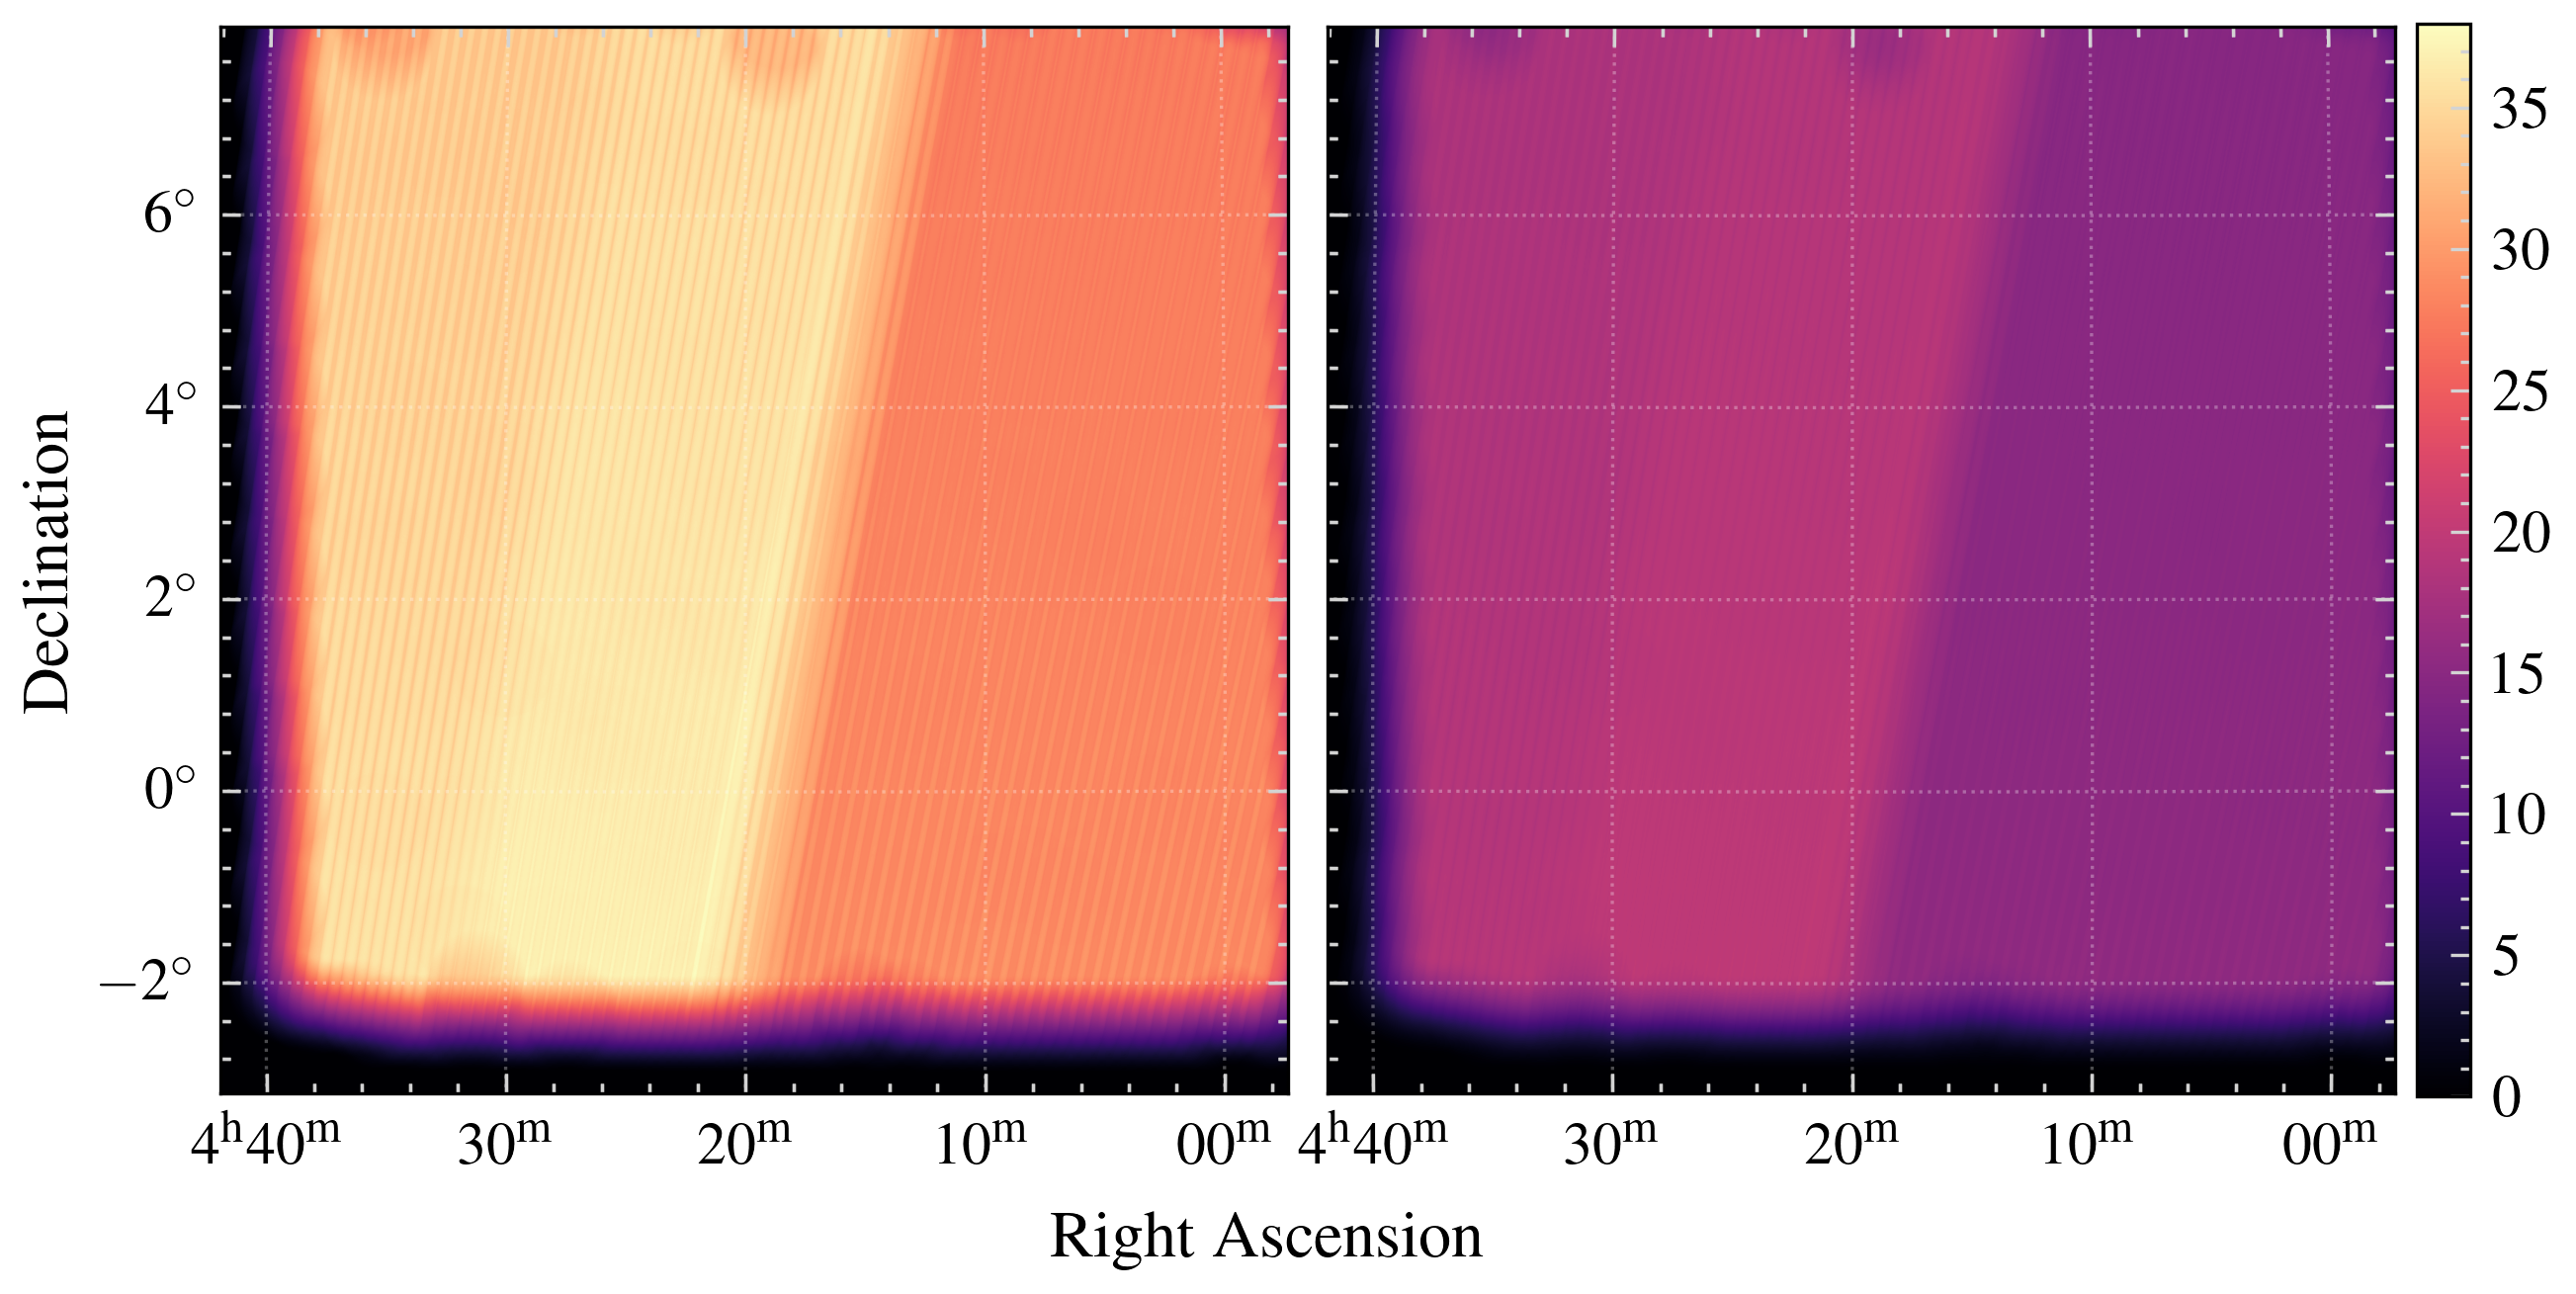
\includegraphics[width=\textwidth]{appendix_a/exposure_map_TM1.png}
    \caption[Exposure maps for TM1.]{Soft-bad exposure map for TM1 created in Section \ref{sec:exposure_map}. \textit{Left:} flat exposure map. \textit{Right:} vignetted exposure map. The color bar units are seconds.}
    \label{fig:TM1}
\end{figure}

\begin{figure}[htbp]
    \centering
    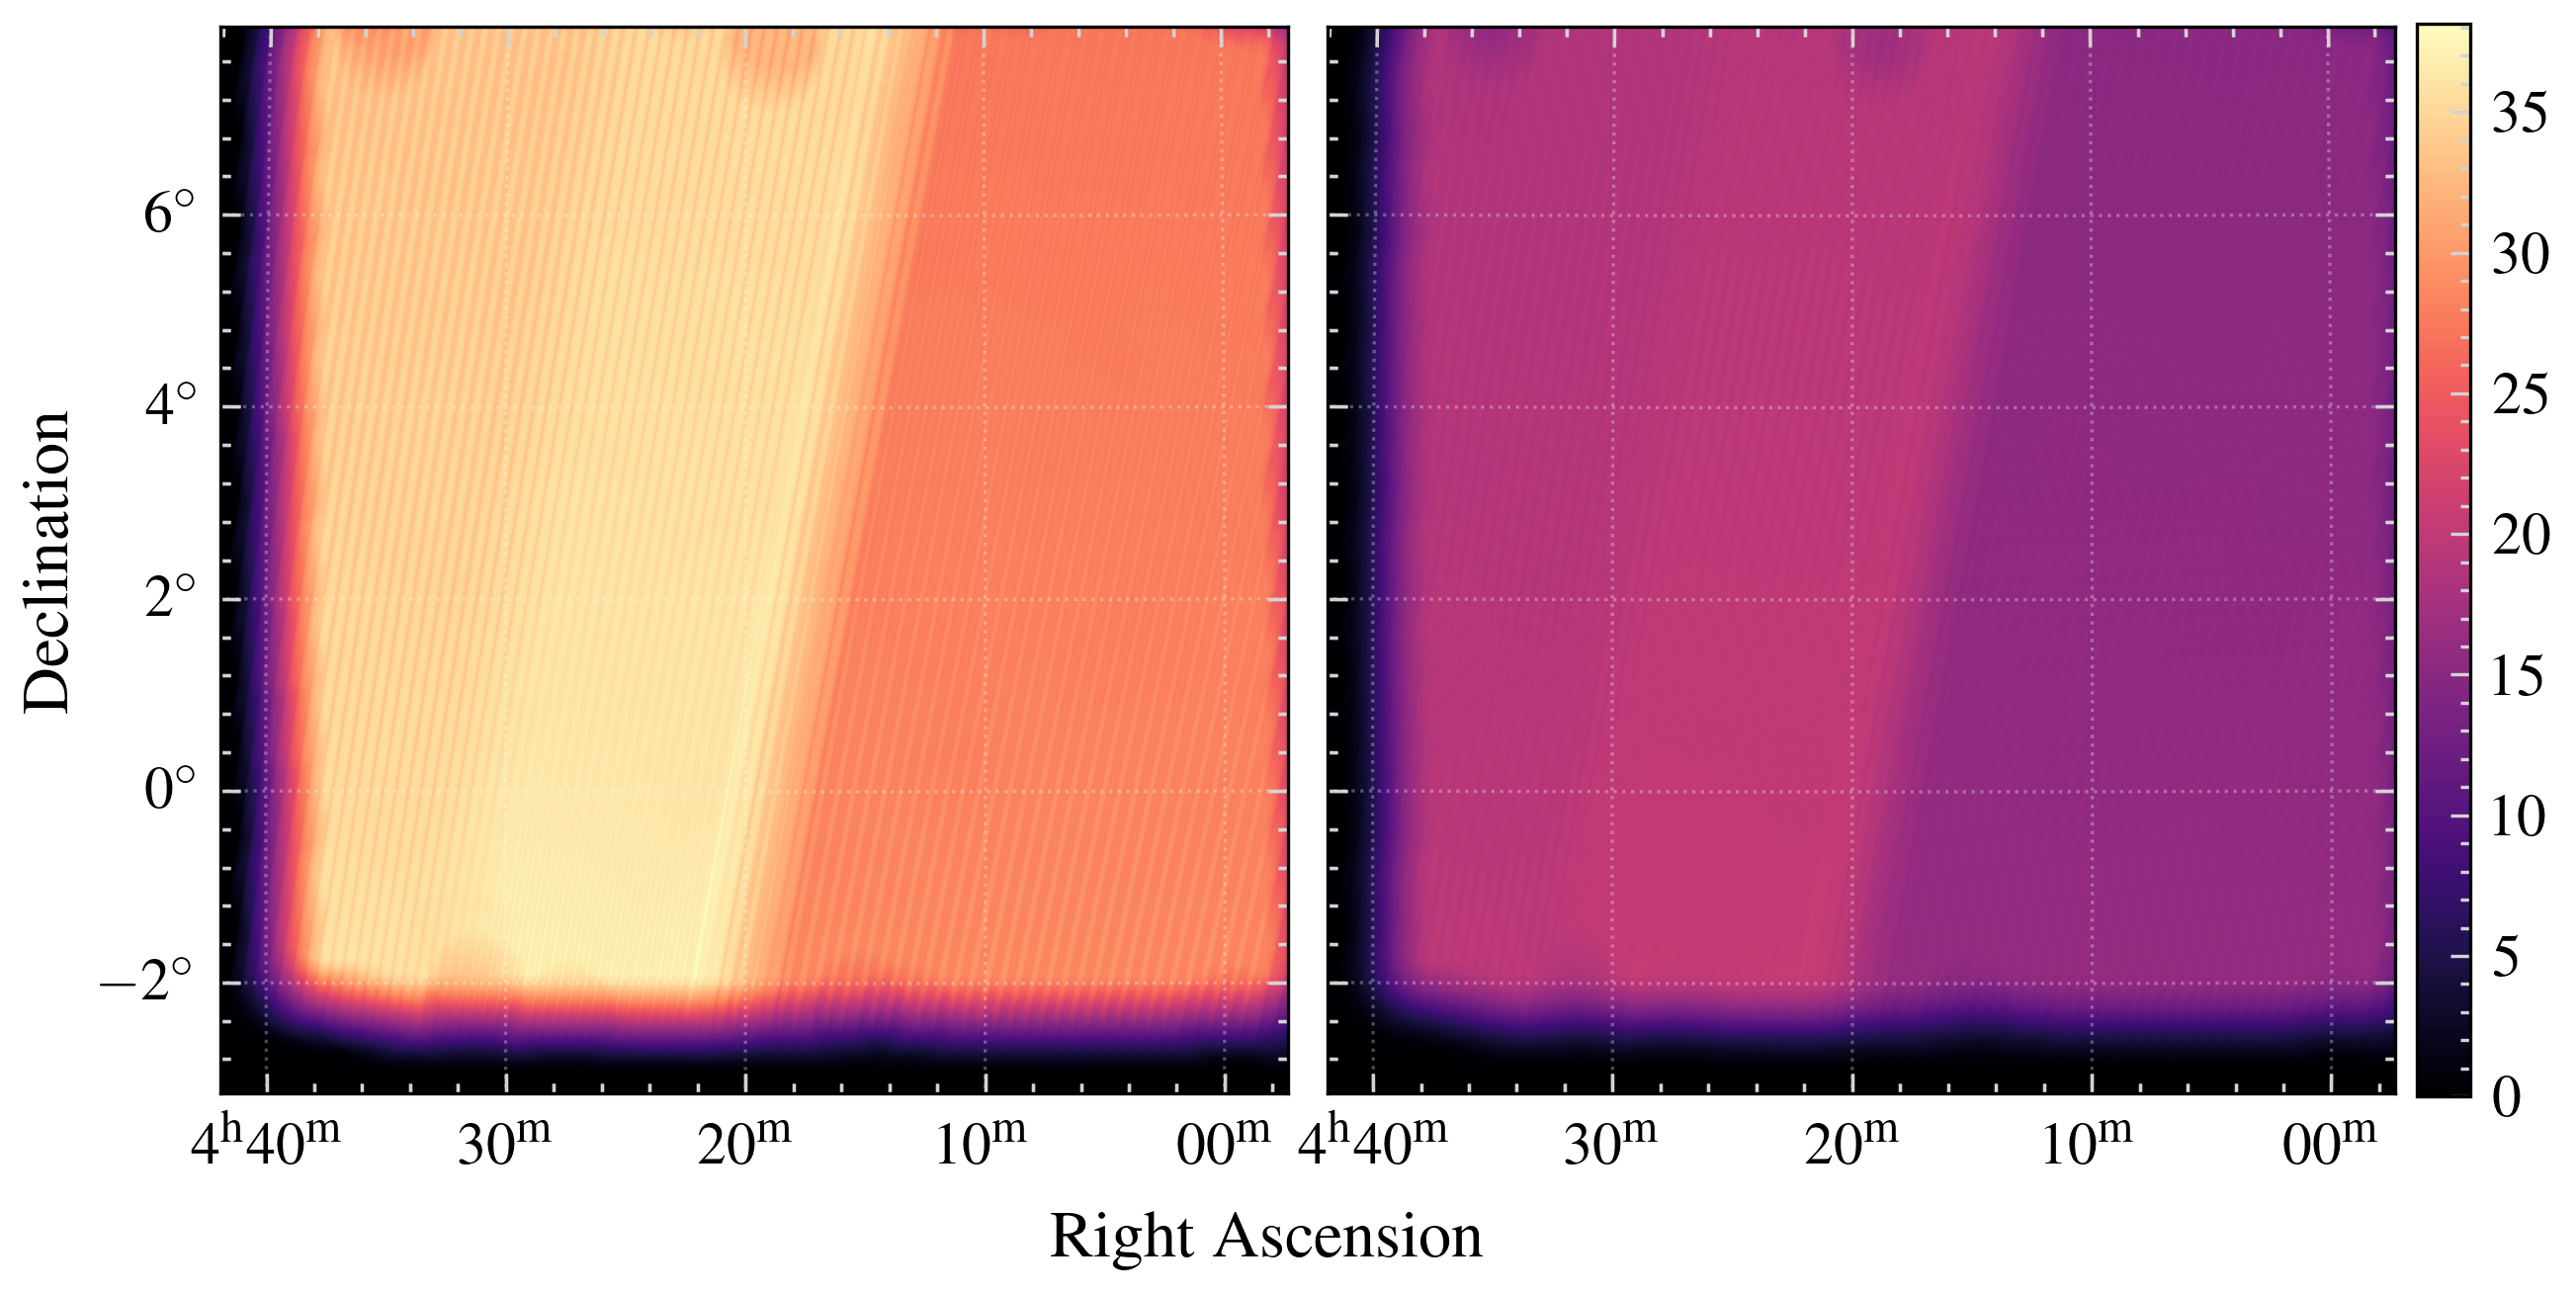
\includegraphics[width=\textwidth]{appendix_a/exposure_map_TM2.png}
    \caption[Exposure maps for TM2.]{Soft-bad exposure map for TM2 created in Section \ref{sec:exposure_map}. \textit{Left:} flat exposure map. \textit{Right:} vignetted exposure map. The color bar units are seconds.}
    \label{fig:TM2}
\end{figure}

\begin{figure}[htbp]
    \centering
    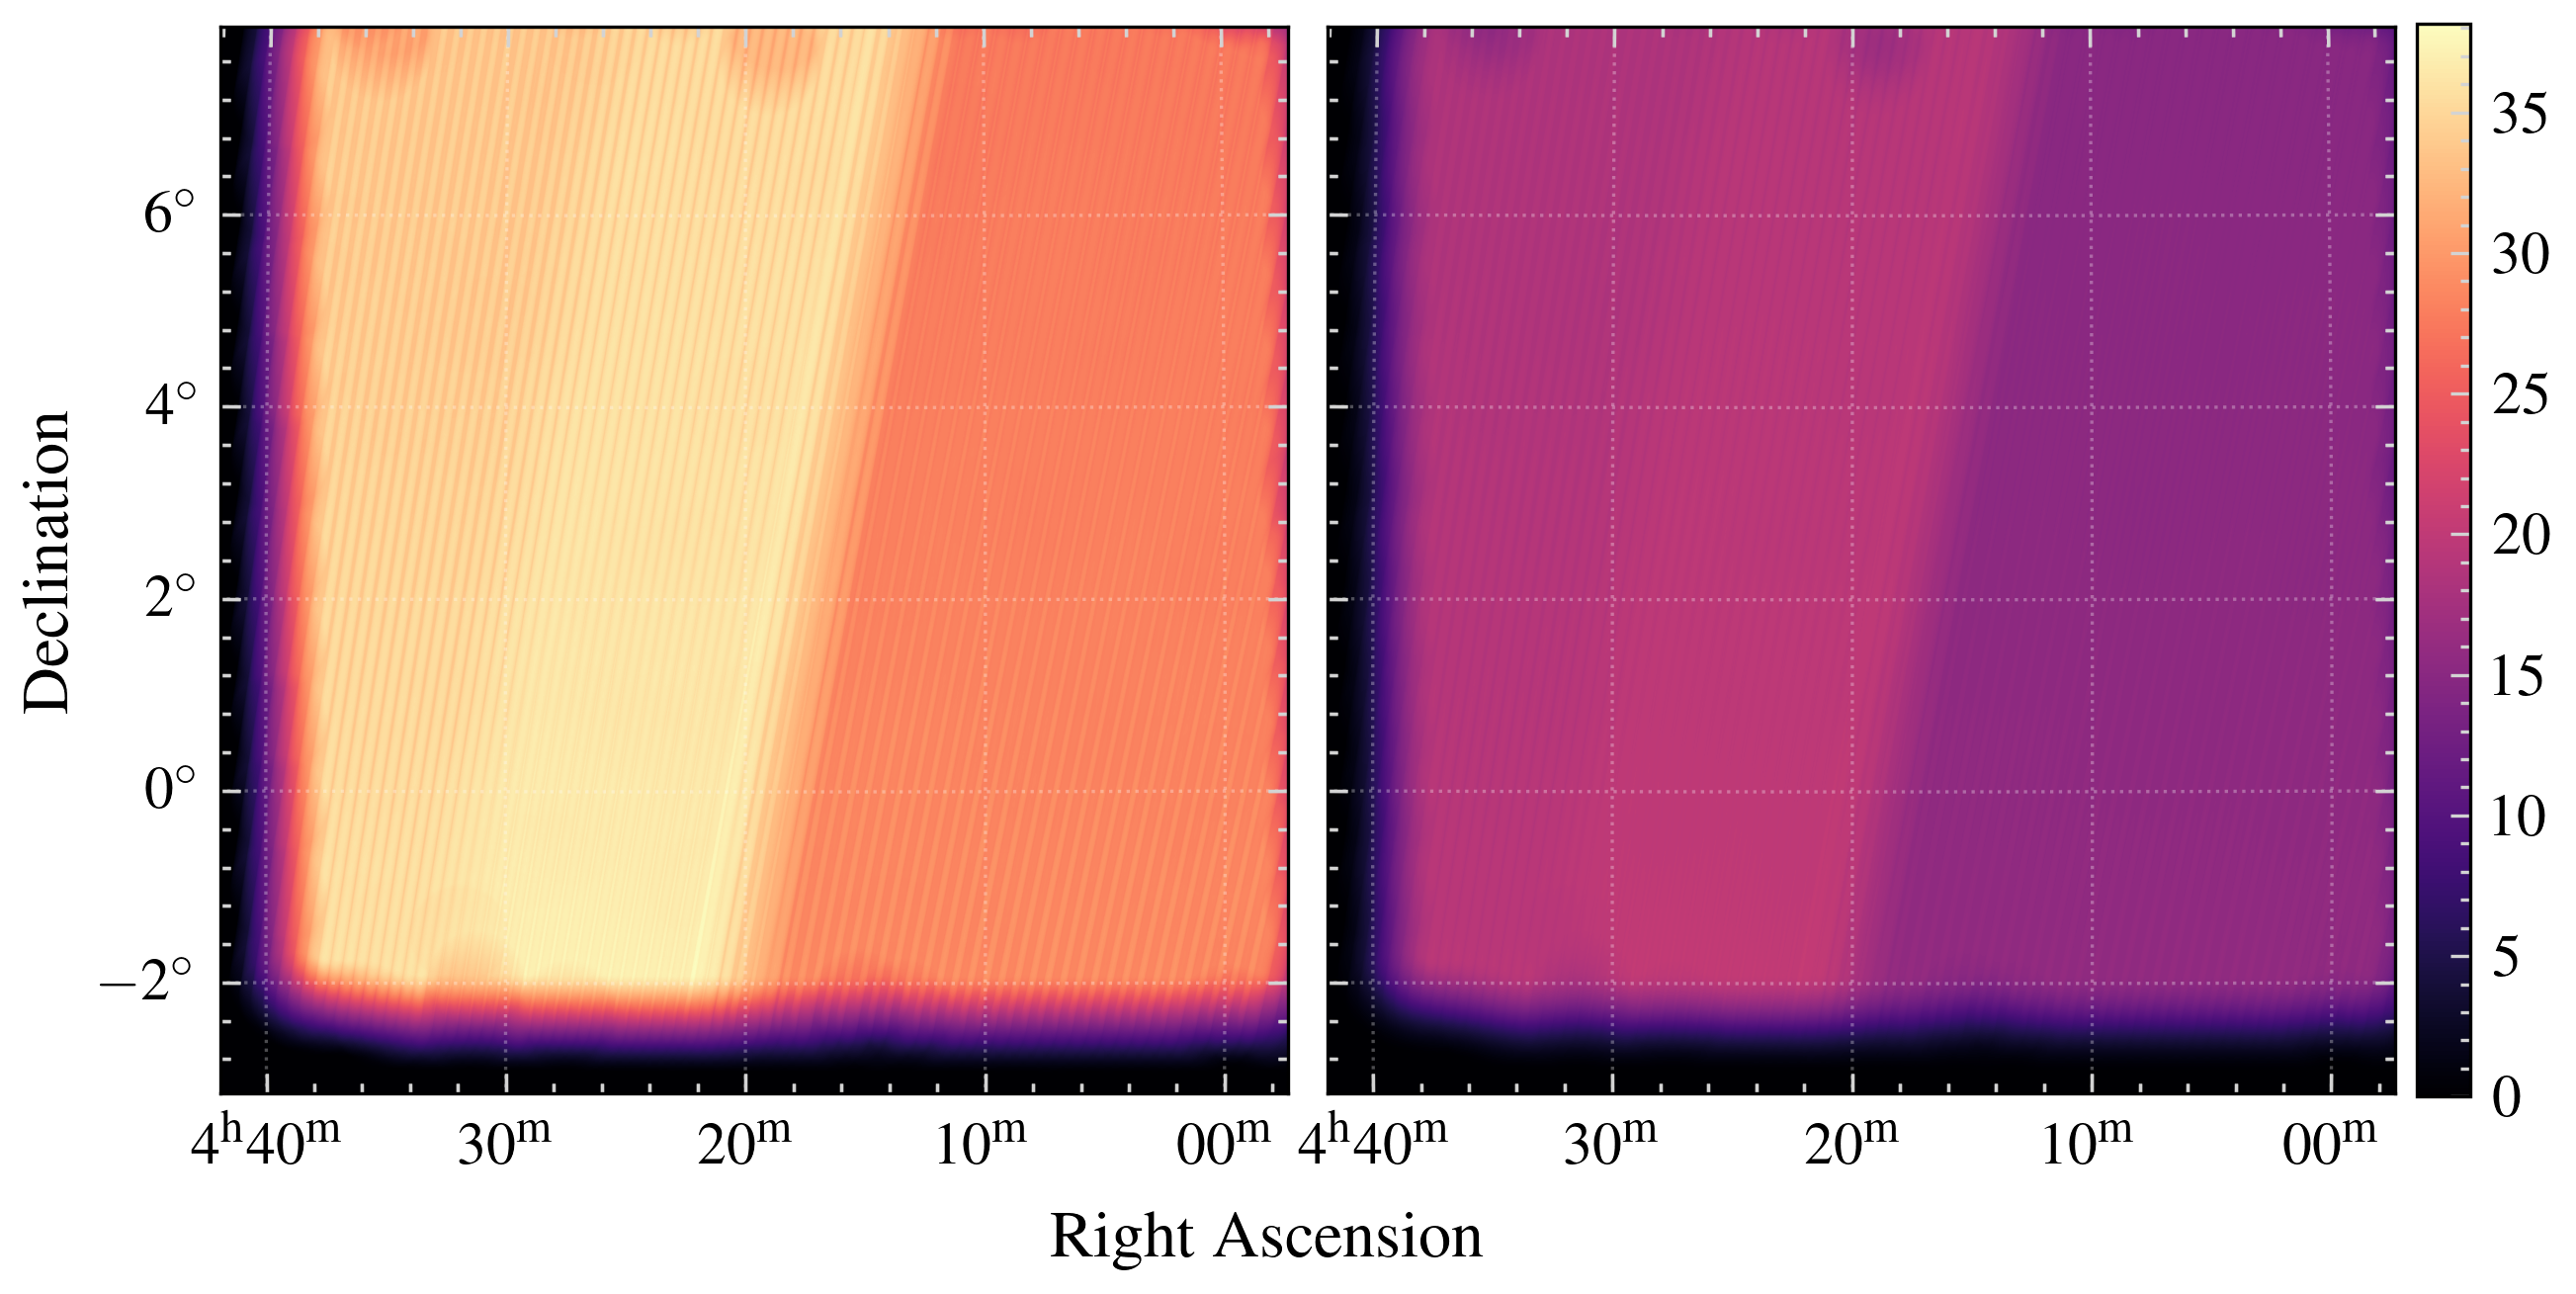
\includegraphics[width=\textwidth]{appendix_a/exposure_map_TM3.png}
    \caption[Exposure maps for TM3.]{Soft-bad exposure map for TM3 created in Section \ref{sec:exposure_map}. \textit{Left:} flat exposure map. \textit{Right:} vignetted exposure map. The color bar units are seconds.}
    \label{fig:TM3}
\end{figure}

\begin{figure}[htbp]
    \centering
    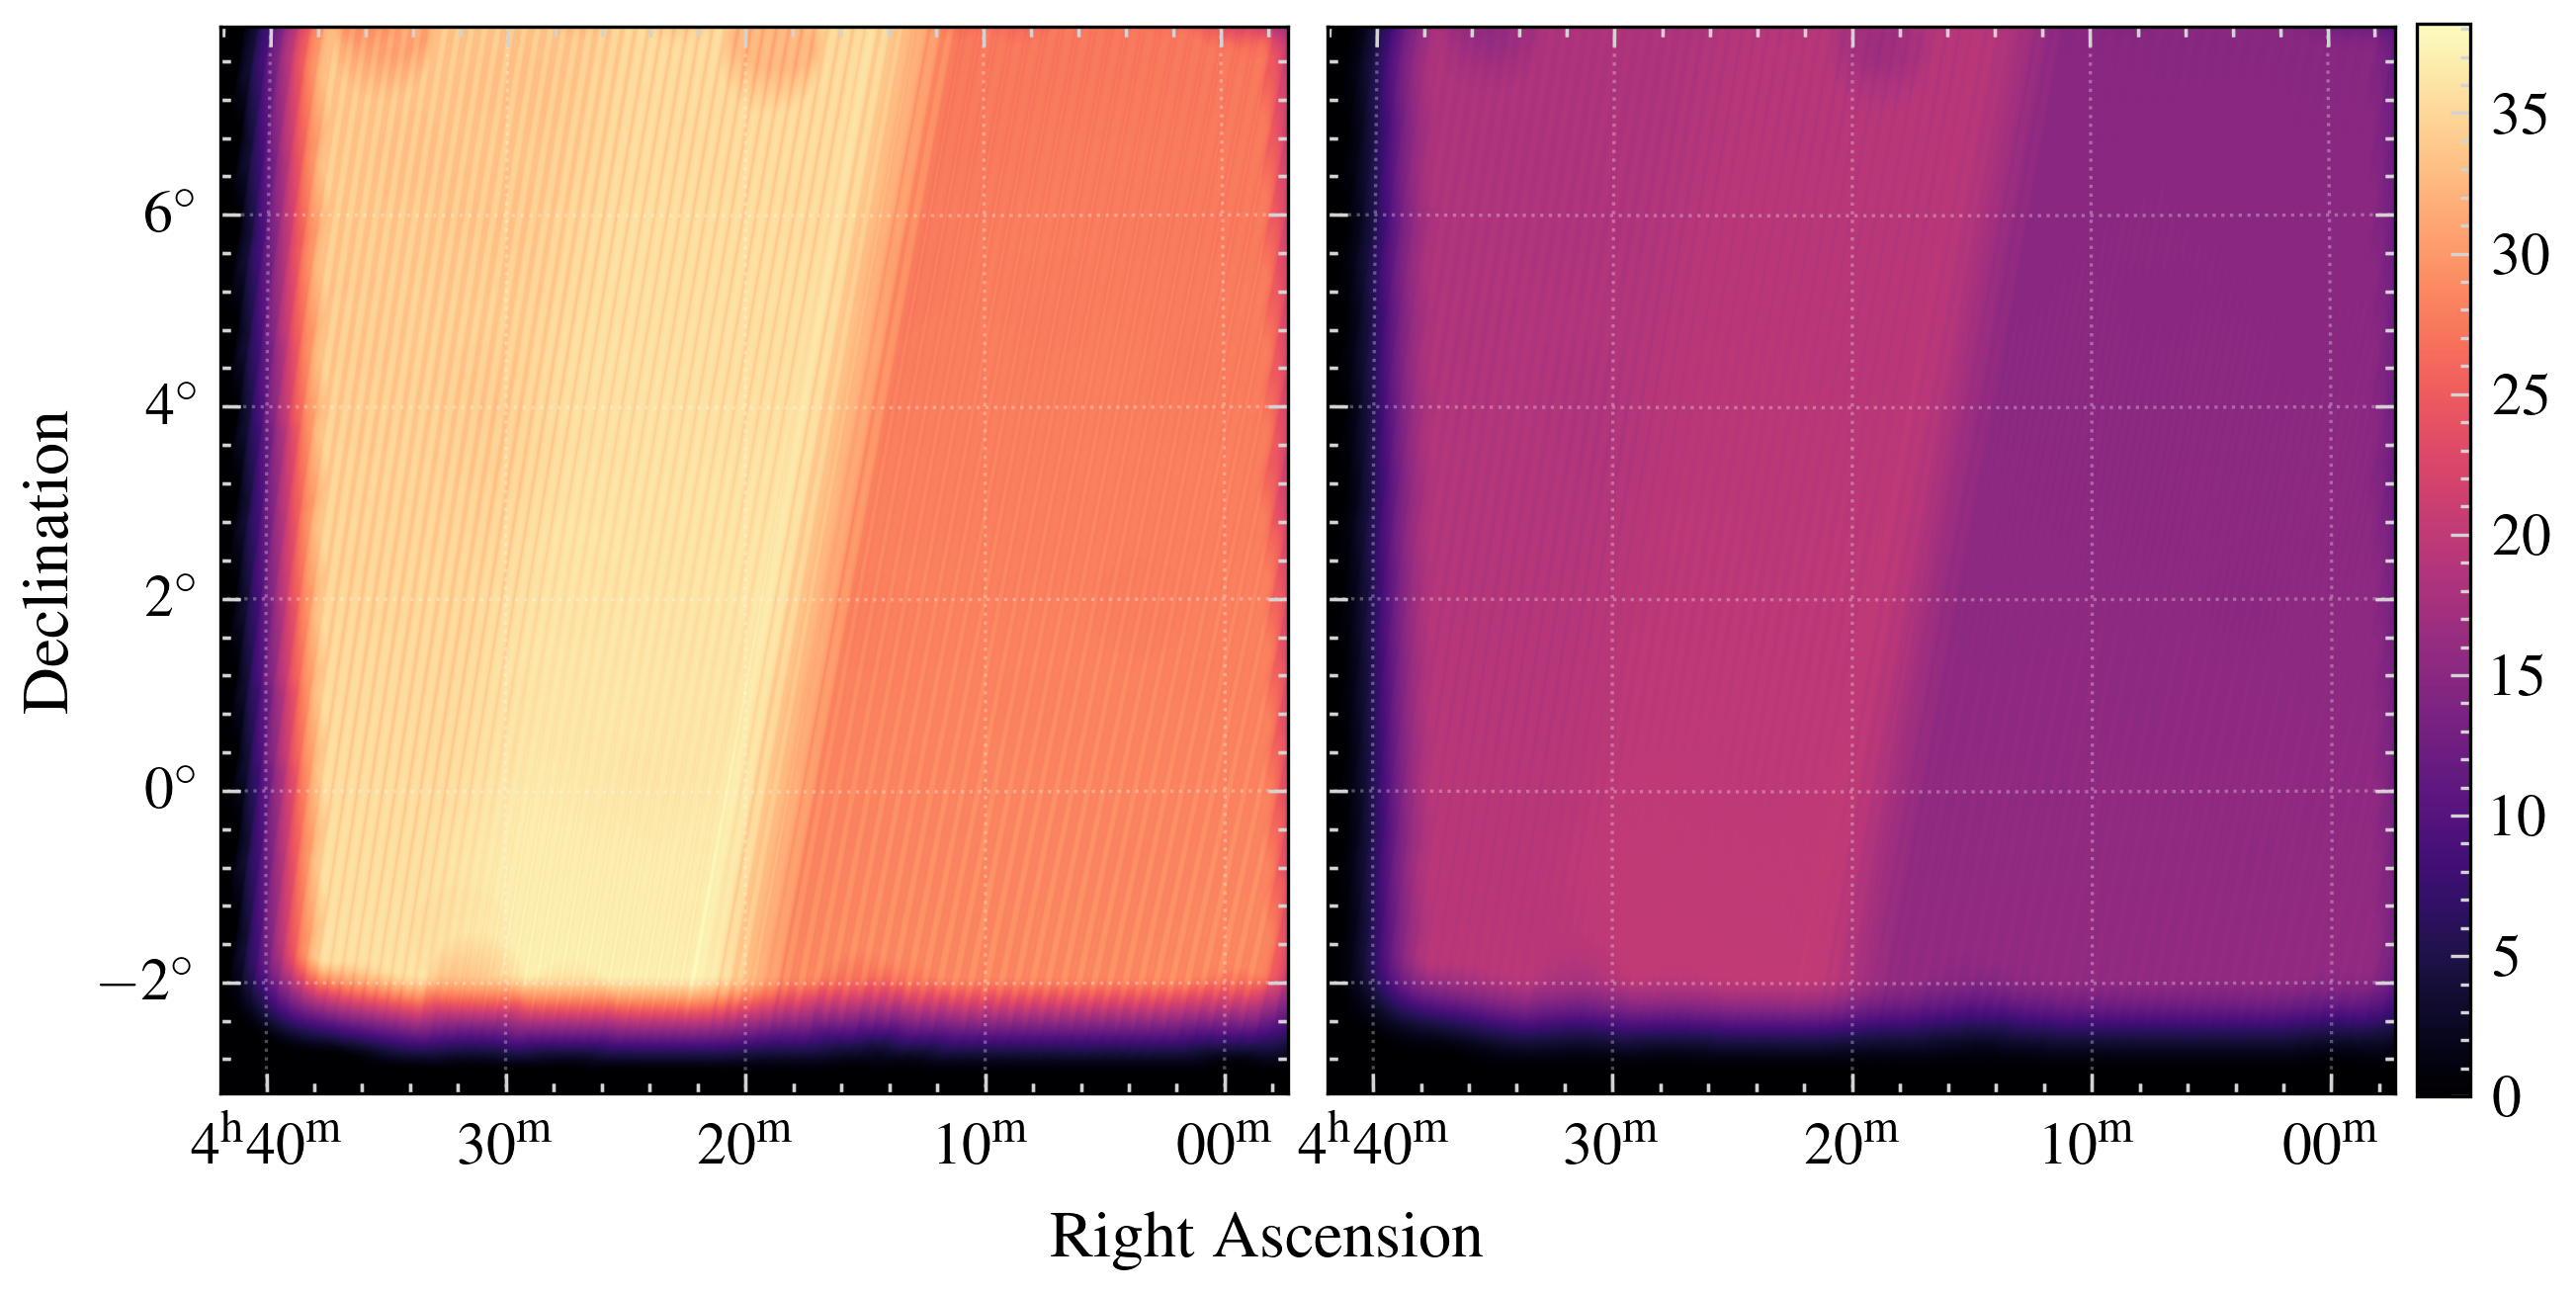
\includegraphics[width=\textwidth]{appendix_a/exposure_map_TM4.png}
    \caption[Exposure maps for TM4.]{Soft-bad exposure map for TM4 created in Section \ref{sec:exposure_map}. \textit{Left:} flat exposure map. \textit{Right:} vignetted exposure map. The color bar units are seconds.}
    \label{fig:TM4}
\end{figure}

\begin{figure}[htbp]
    \centering
    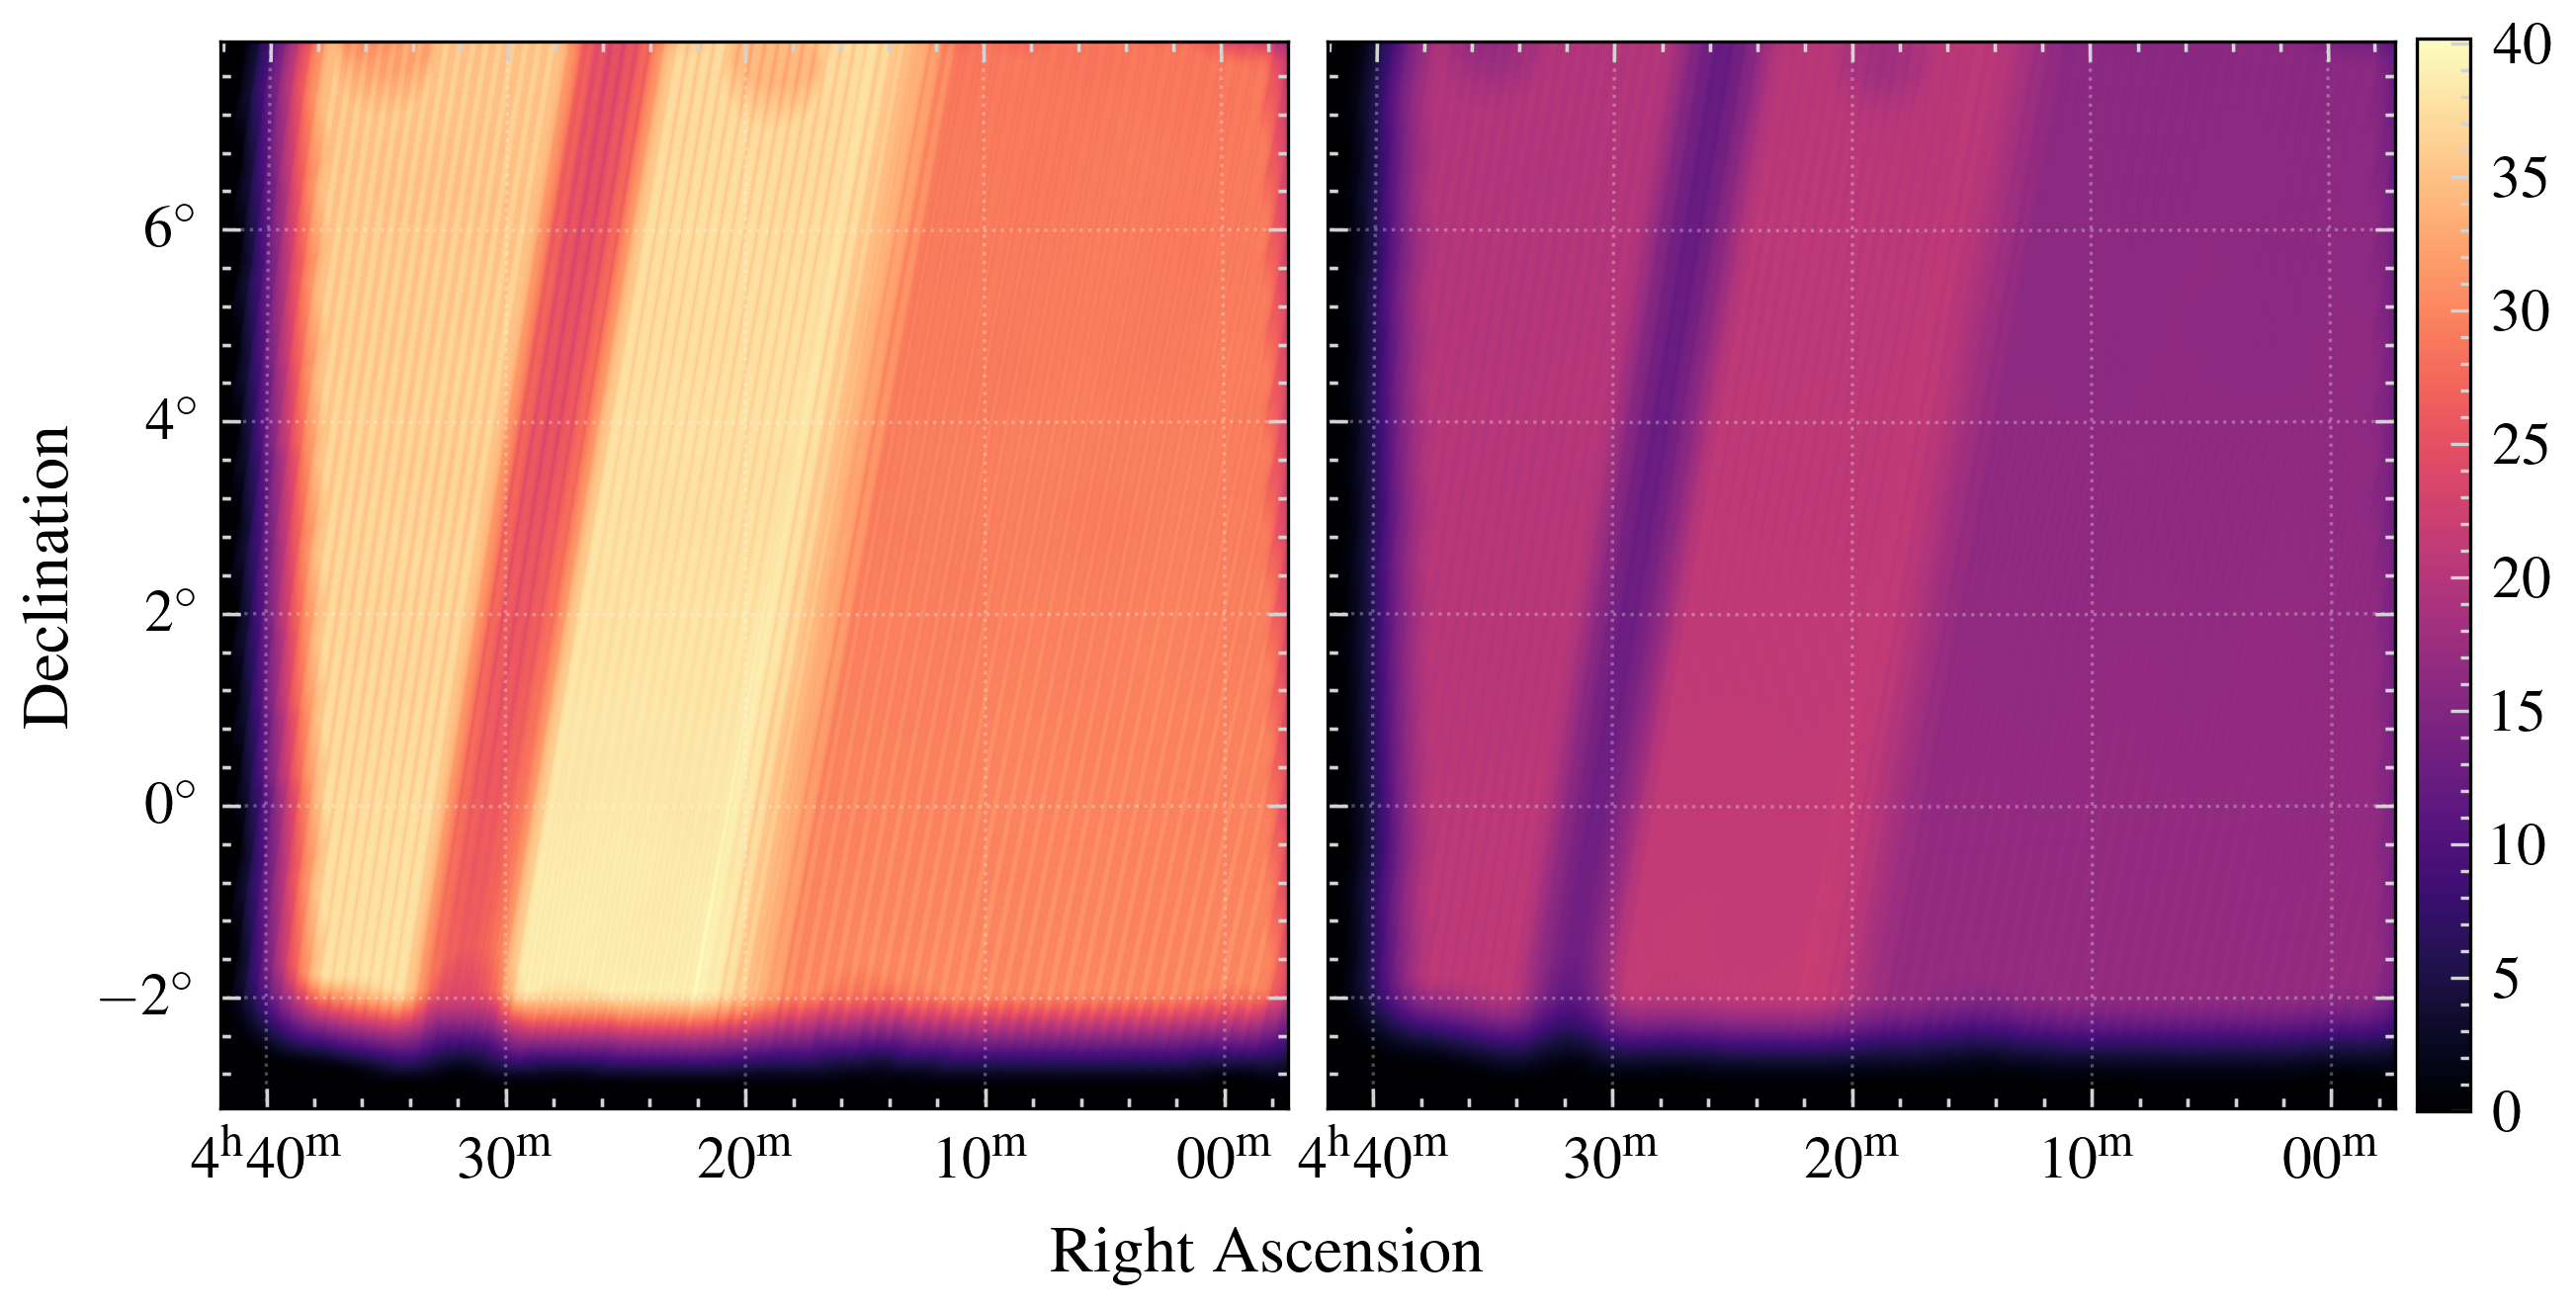
\includegraphics[width=\textwidth]{appendix_a/exposure_map_TM5.png}
    \caption[Exposure maps for TM5.]{Soft-bad exposure map for TM5 created in Section \ref{sec:exposure_map}. \textit{Left:} flat exposure map. \textit{Right:} vignetted exposure map. The color bar units are seconds.}
    \label{fig:TM5}
\end{figure}

\begin{figure}[htbp]
    \centering
    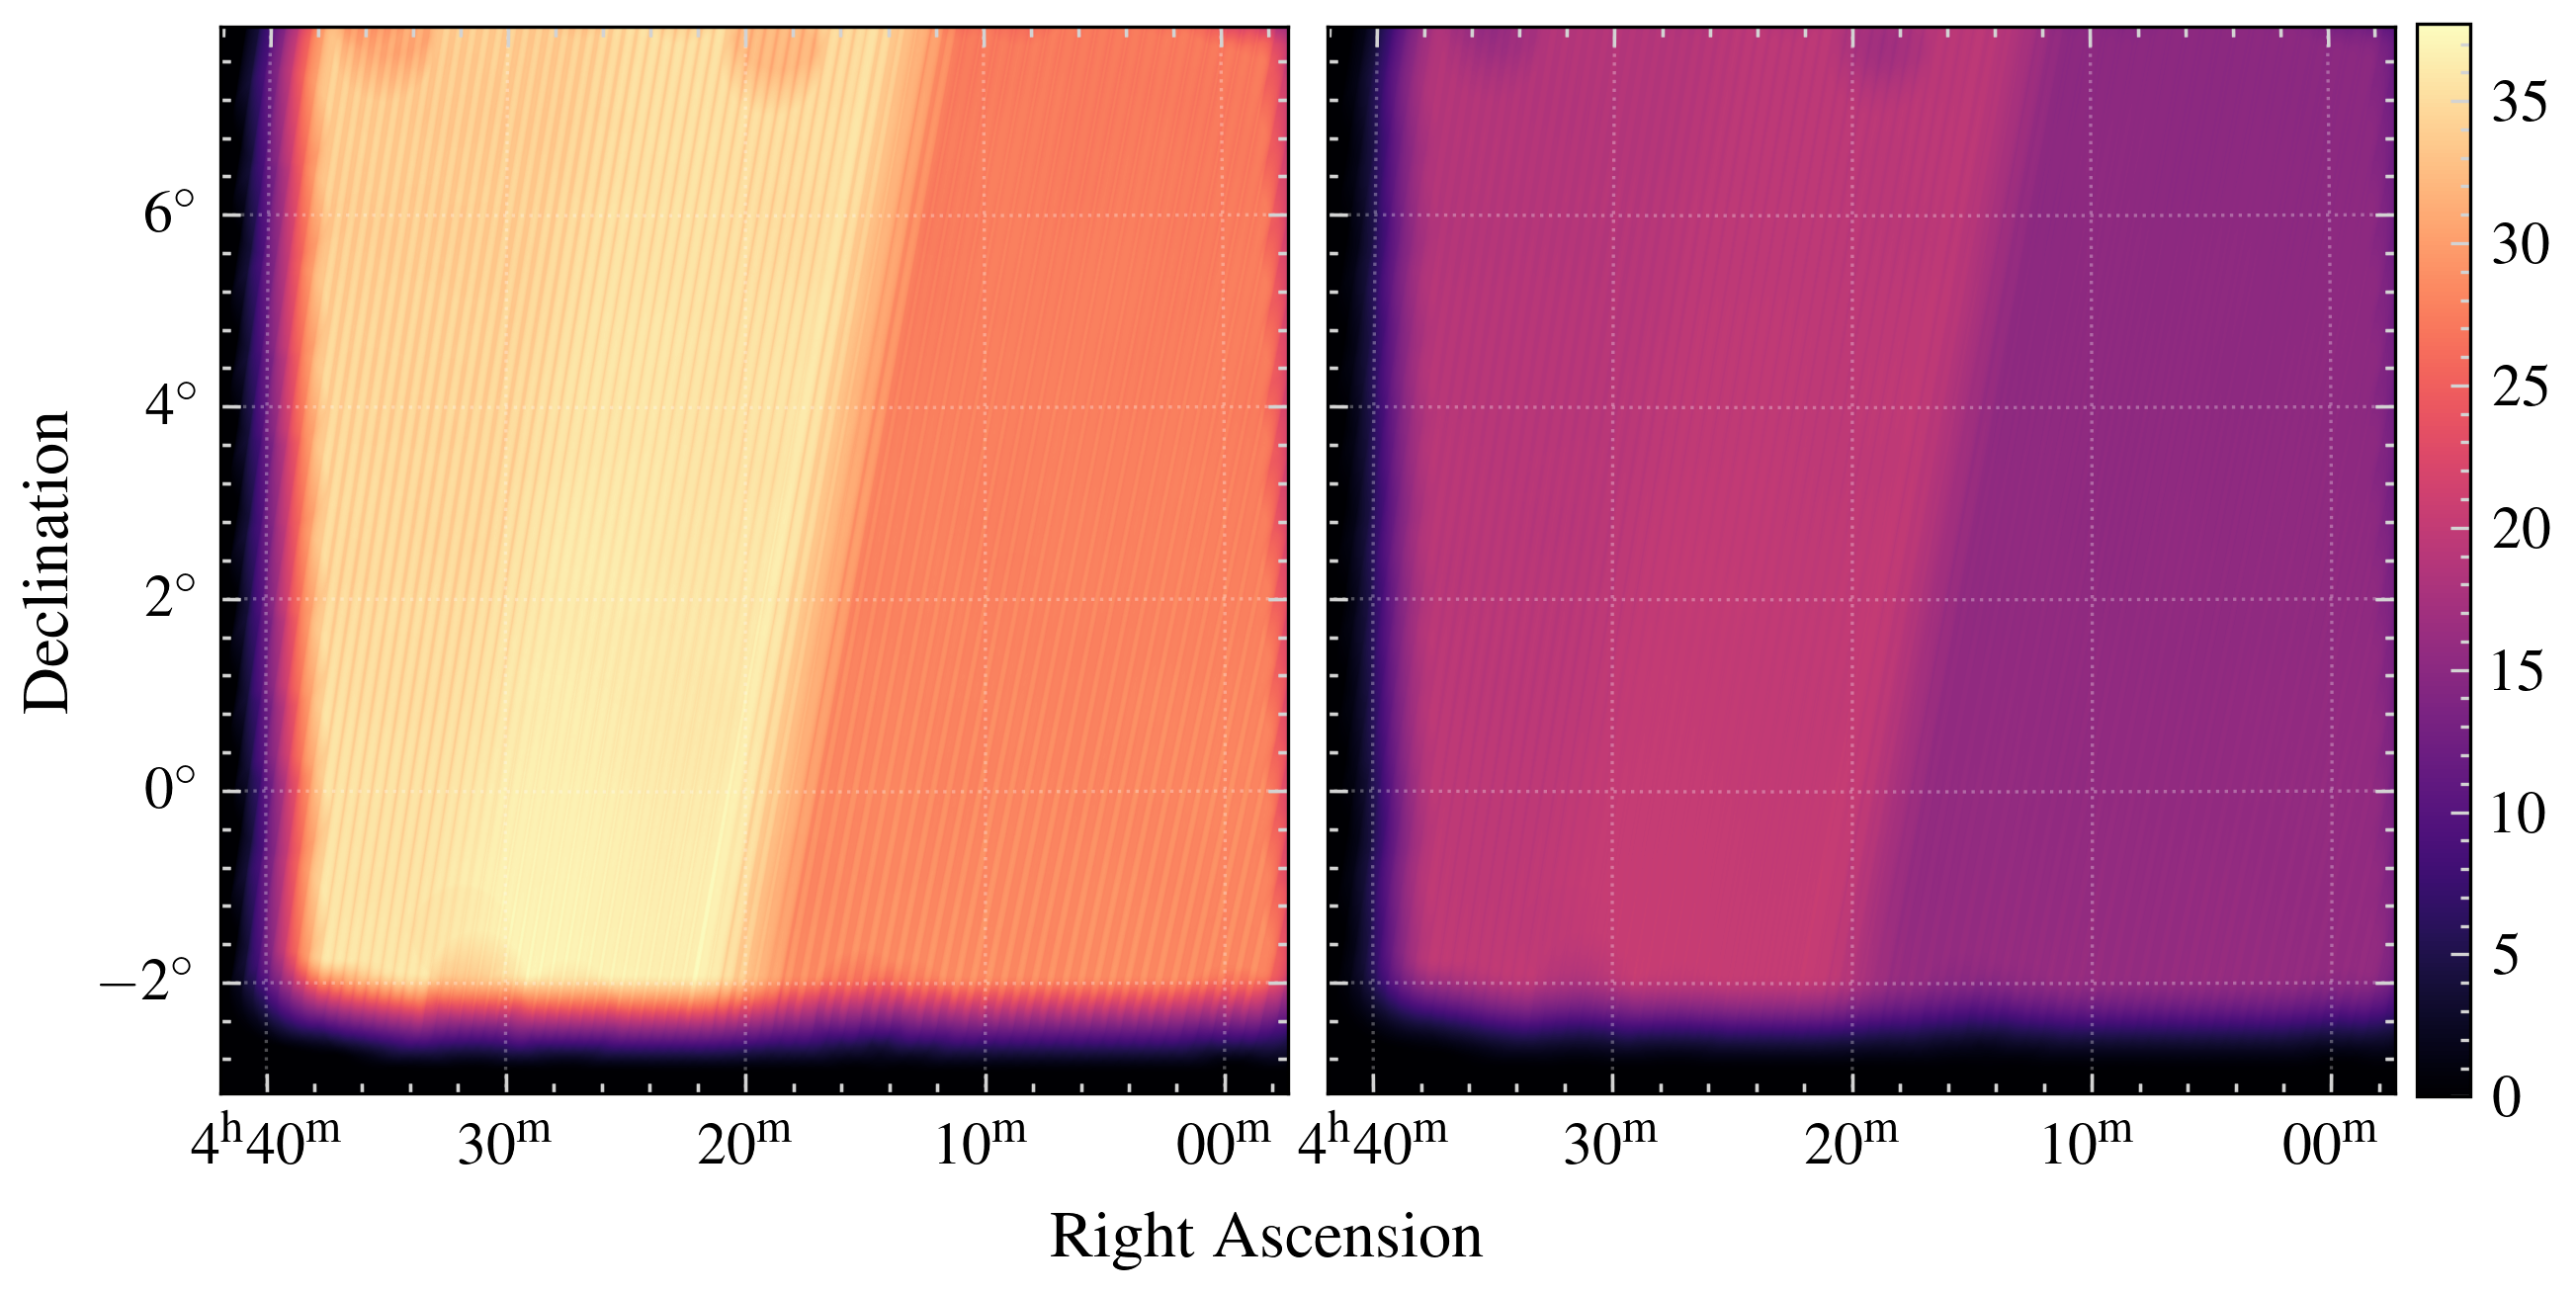
\includegraphics[width=\textwidth]{appendix_a/exposure_map_TM6.png}
    \caption[Exposure maps for TM6.]{Soft-bad exposure map for TM6 created in Section \ref{sec:exposure_map}. \textit{Left:} flat exposure map. \textit{Right:} vignetted exposure map. The color bar units are seconds.}
    \label{fig:TM6}
\end{figure}

\begin{figure}[htbp]
    \centering
    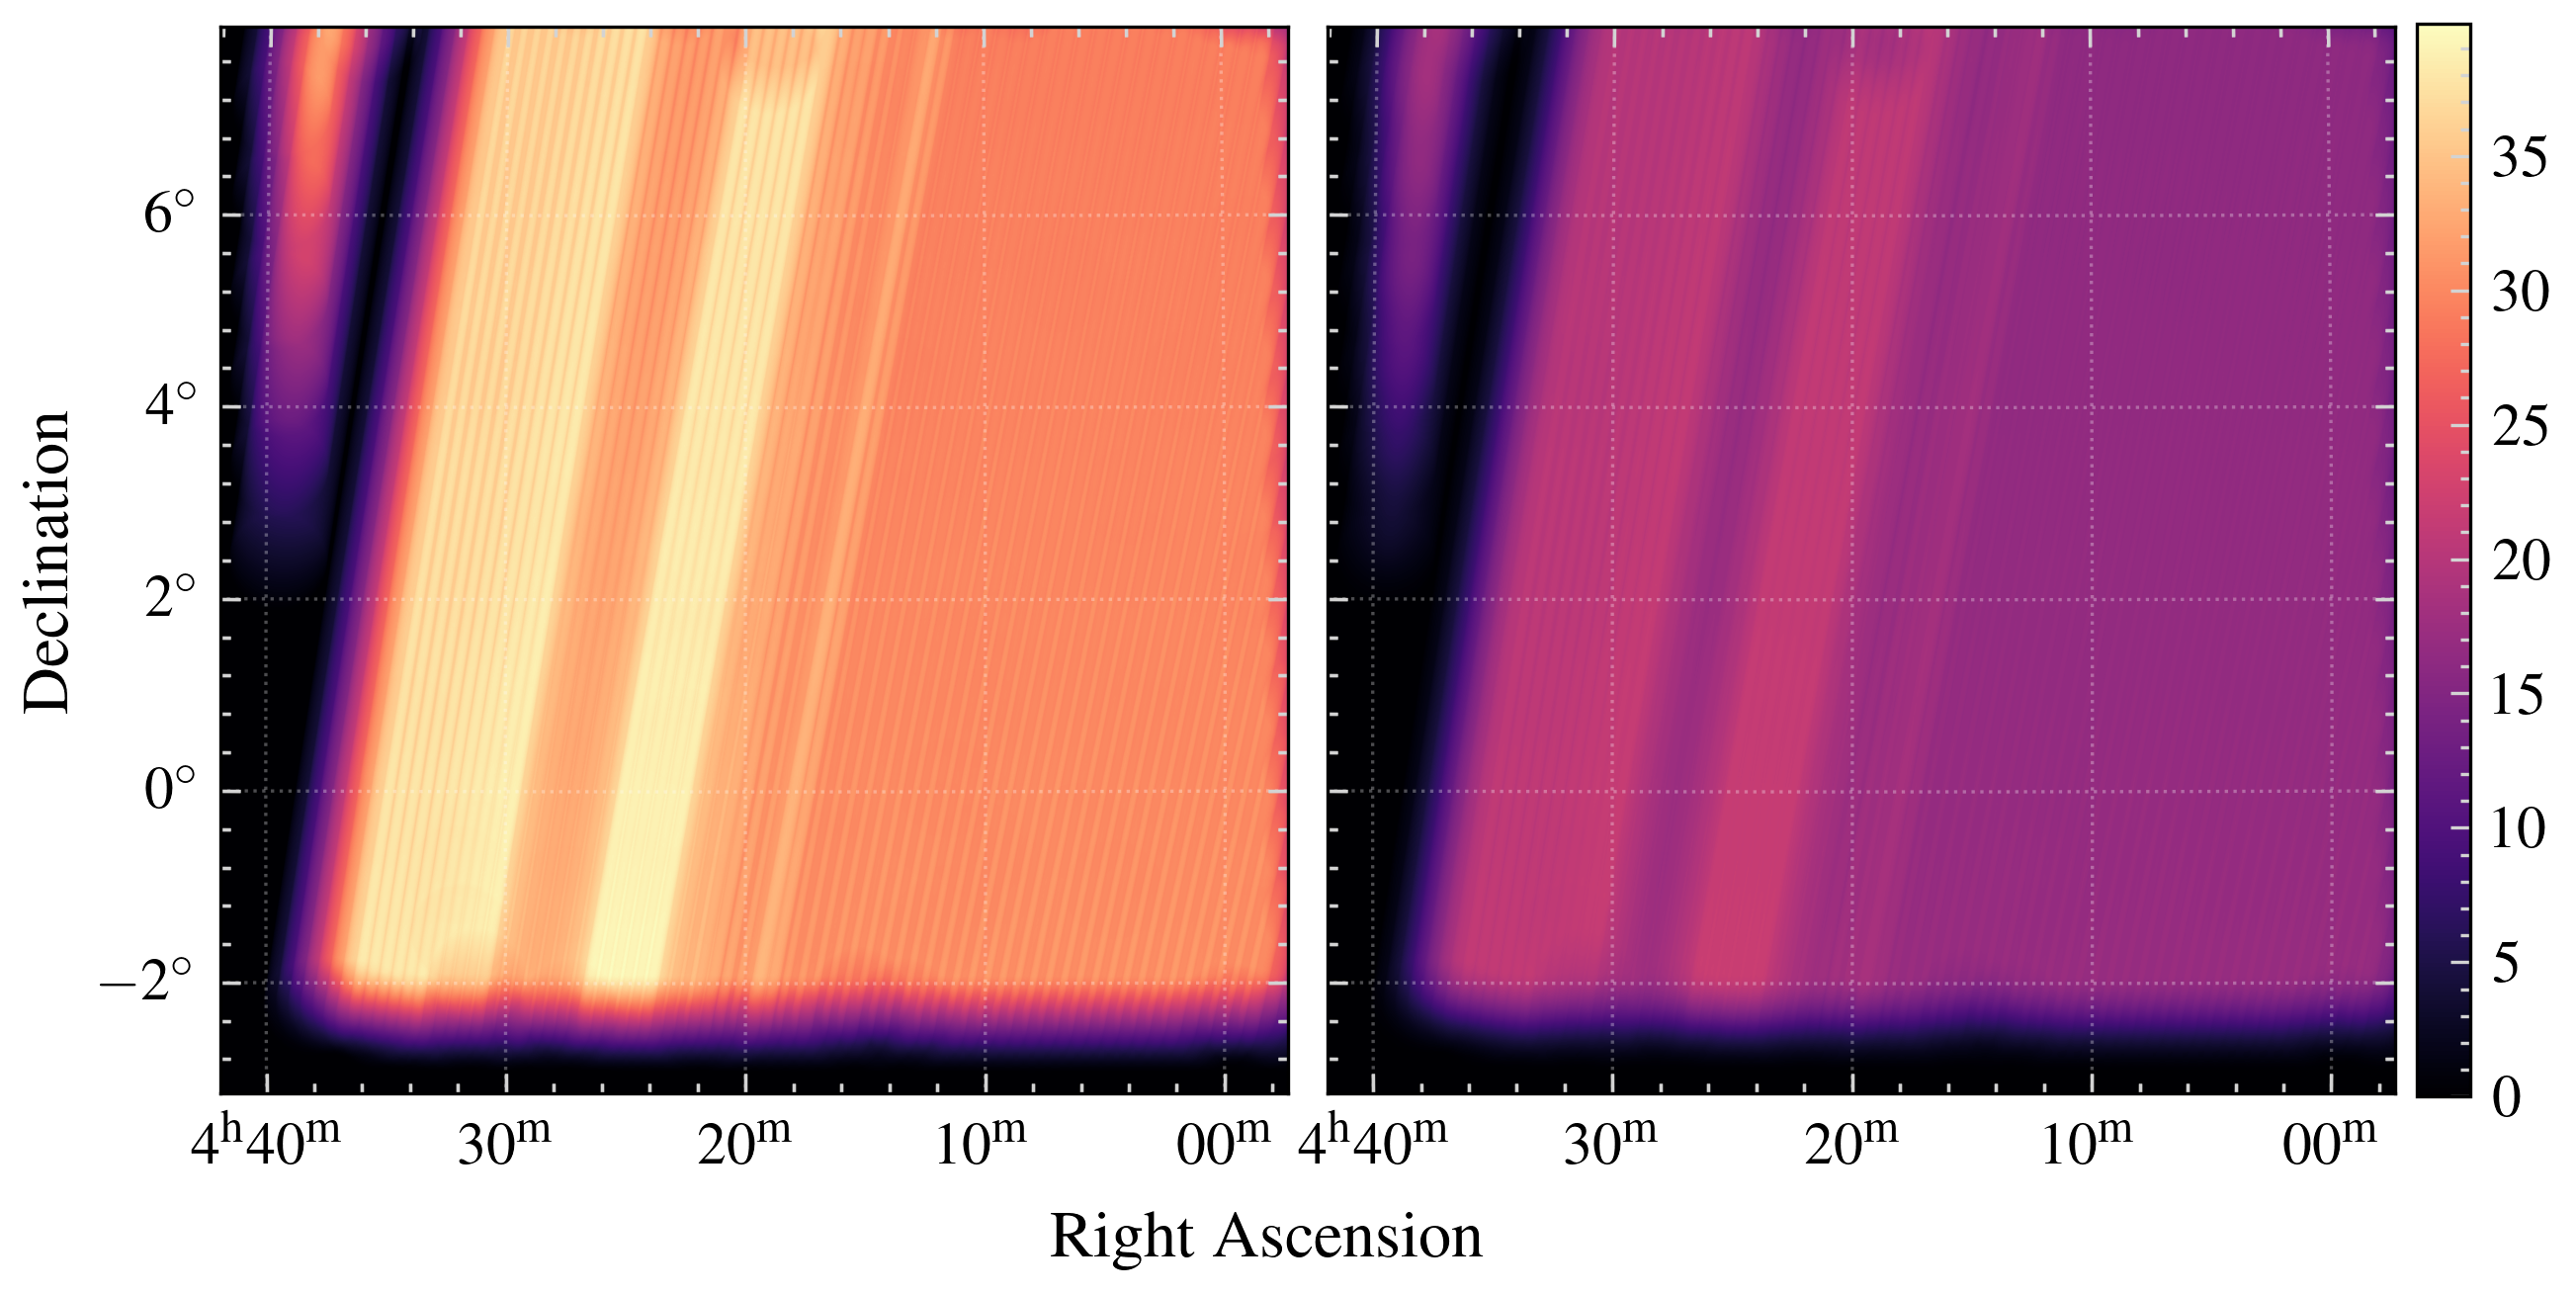
\includegraphics[width=\textwidth]{appendix_a/exposure_map_TM7.png}
    \caption[Exposure maps for TM7.]{Soft-bad exposure map for TM7 created in Section \ref{sec:exposure_map}. \textit{Left:} flat exposure map. \textit{Right:} vignetted exposure map. The color bar units are seconds.}
    \label{fig:TM7}
\end{figure}

\begin{figure}[htbp]
    \centering
    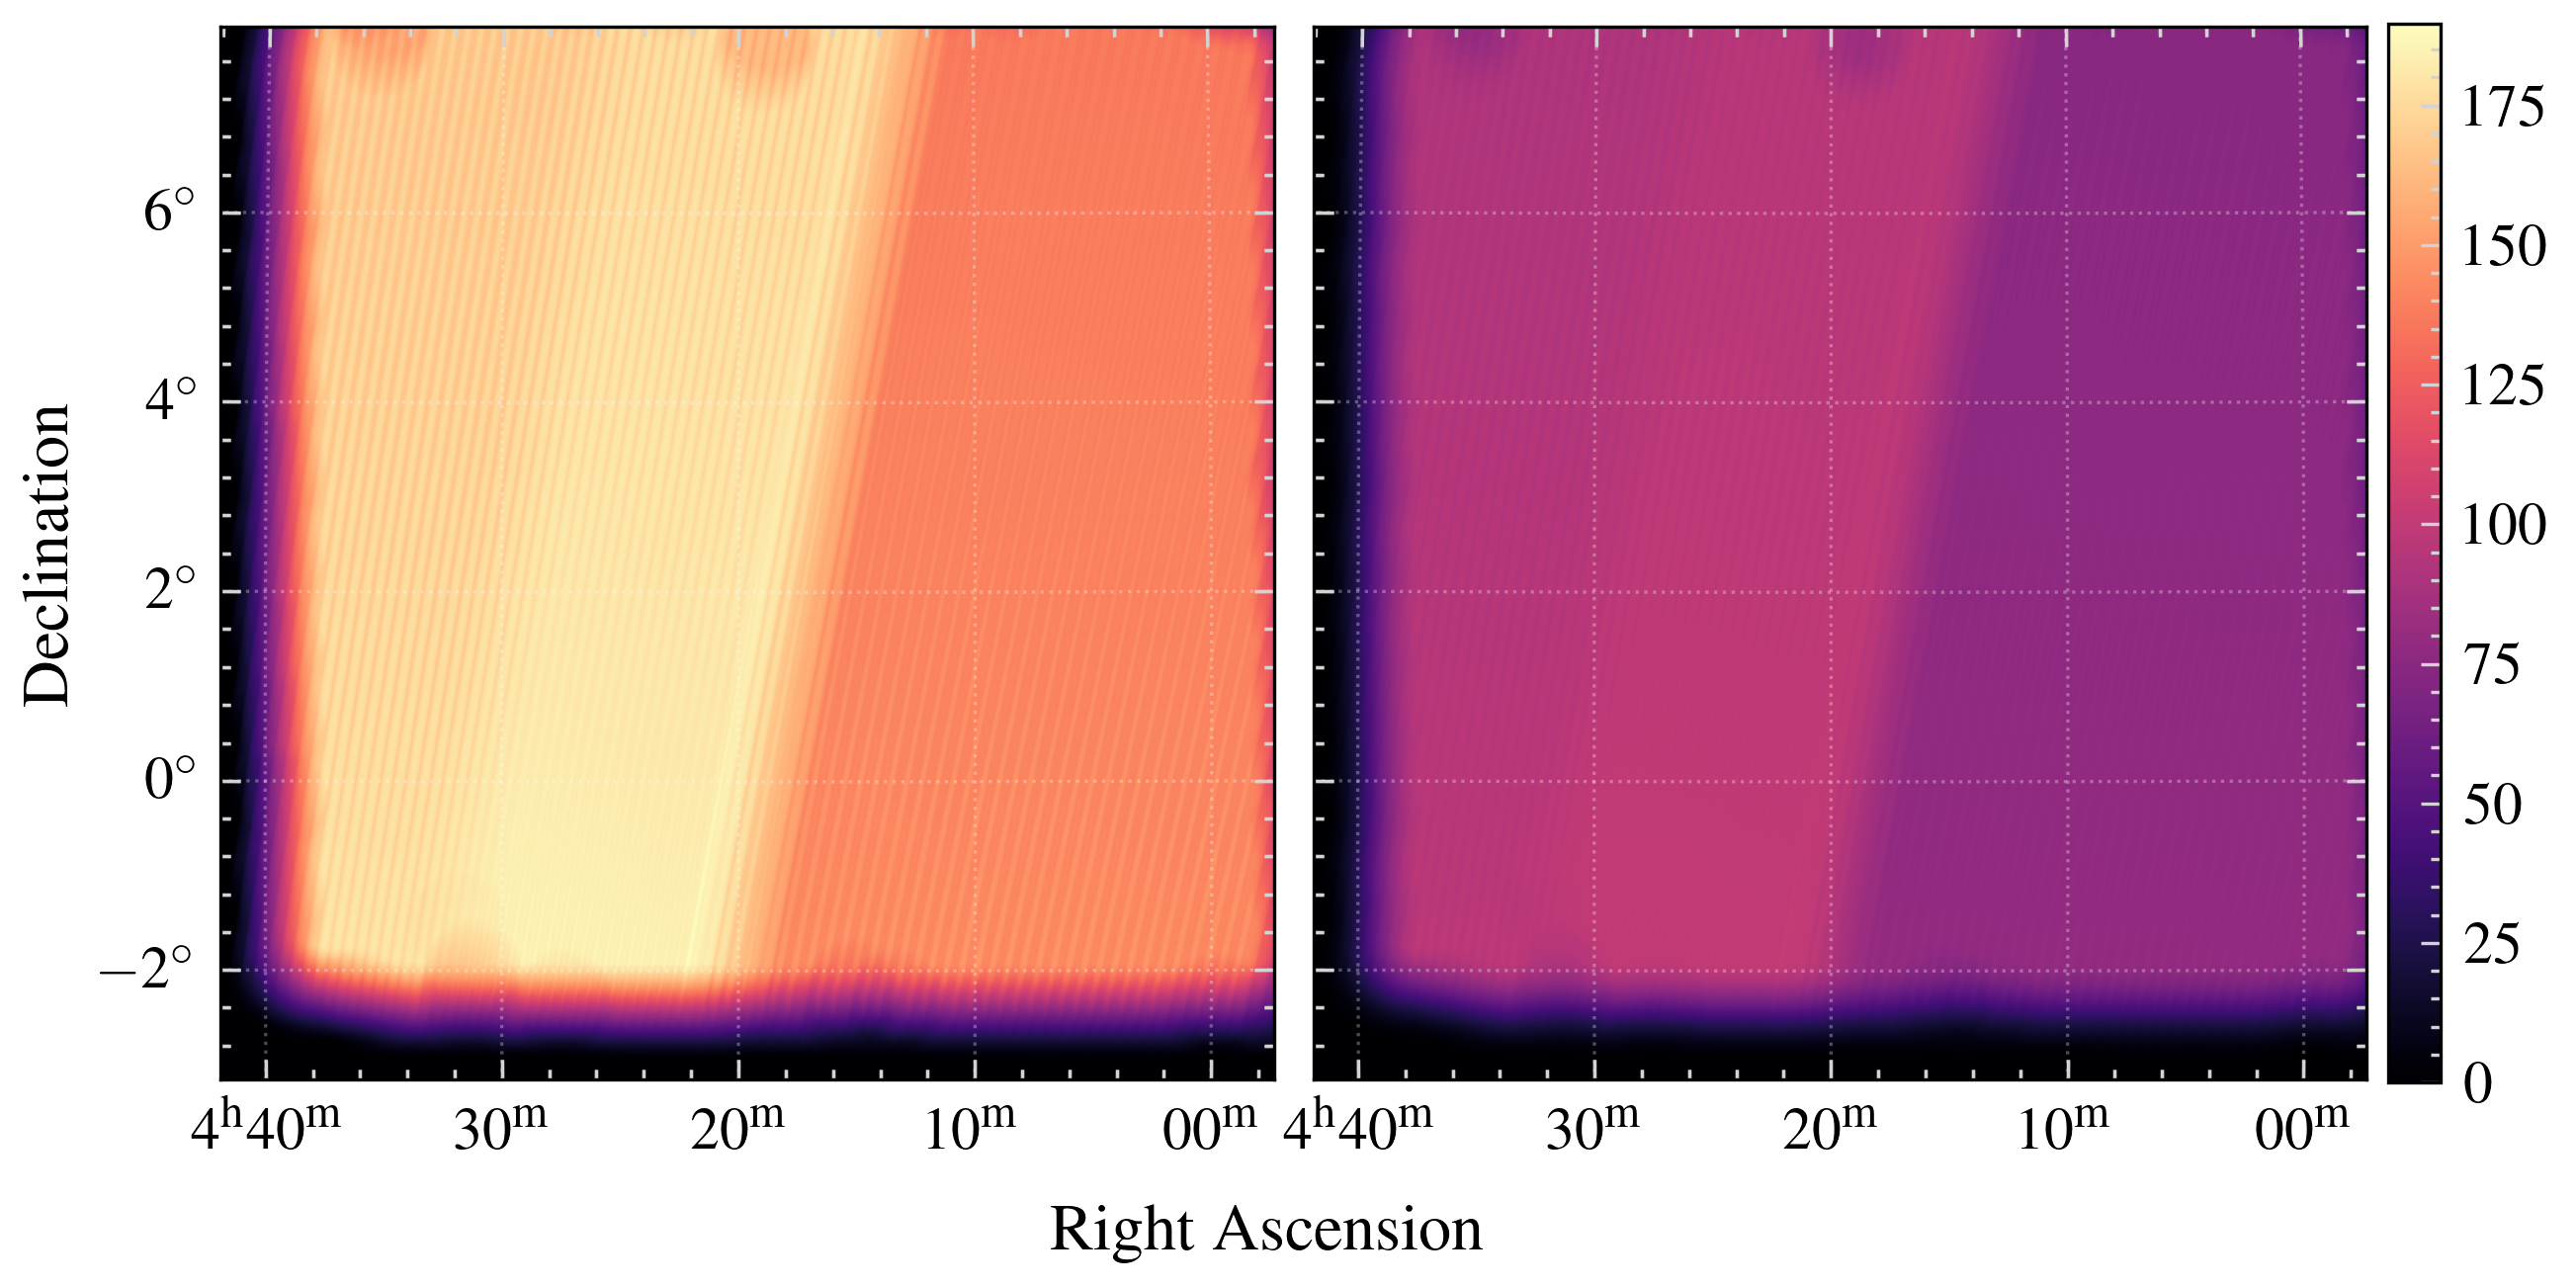
\includegraphics[width=\textwidth]{appendix_a/exposure_map_TM8.png}
    \caption[Exposure maps for TM8.]{Soft-bad exposure map for TM8 created in Section \ref{sec:exposure_map}. \textit{Left:} flat exposure map. \textit{Right:} vignetted exposure map. The color bar units are seconds.}
    \label{fig:TM8}
\end{figure}

\begin{figure}[htbp]
    \centering
    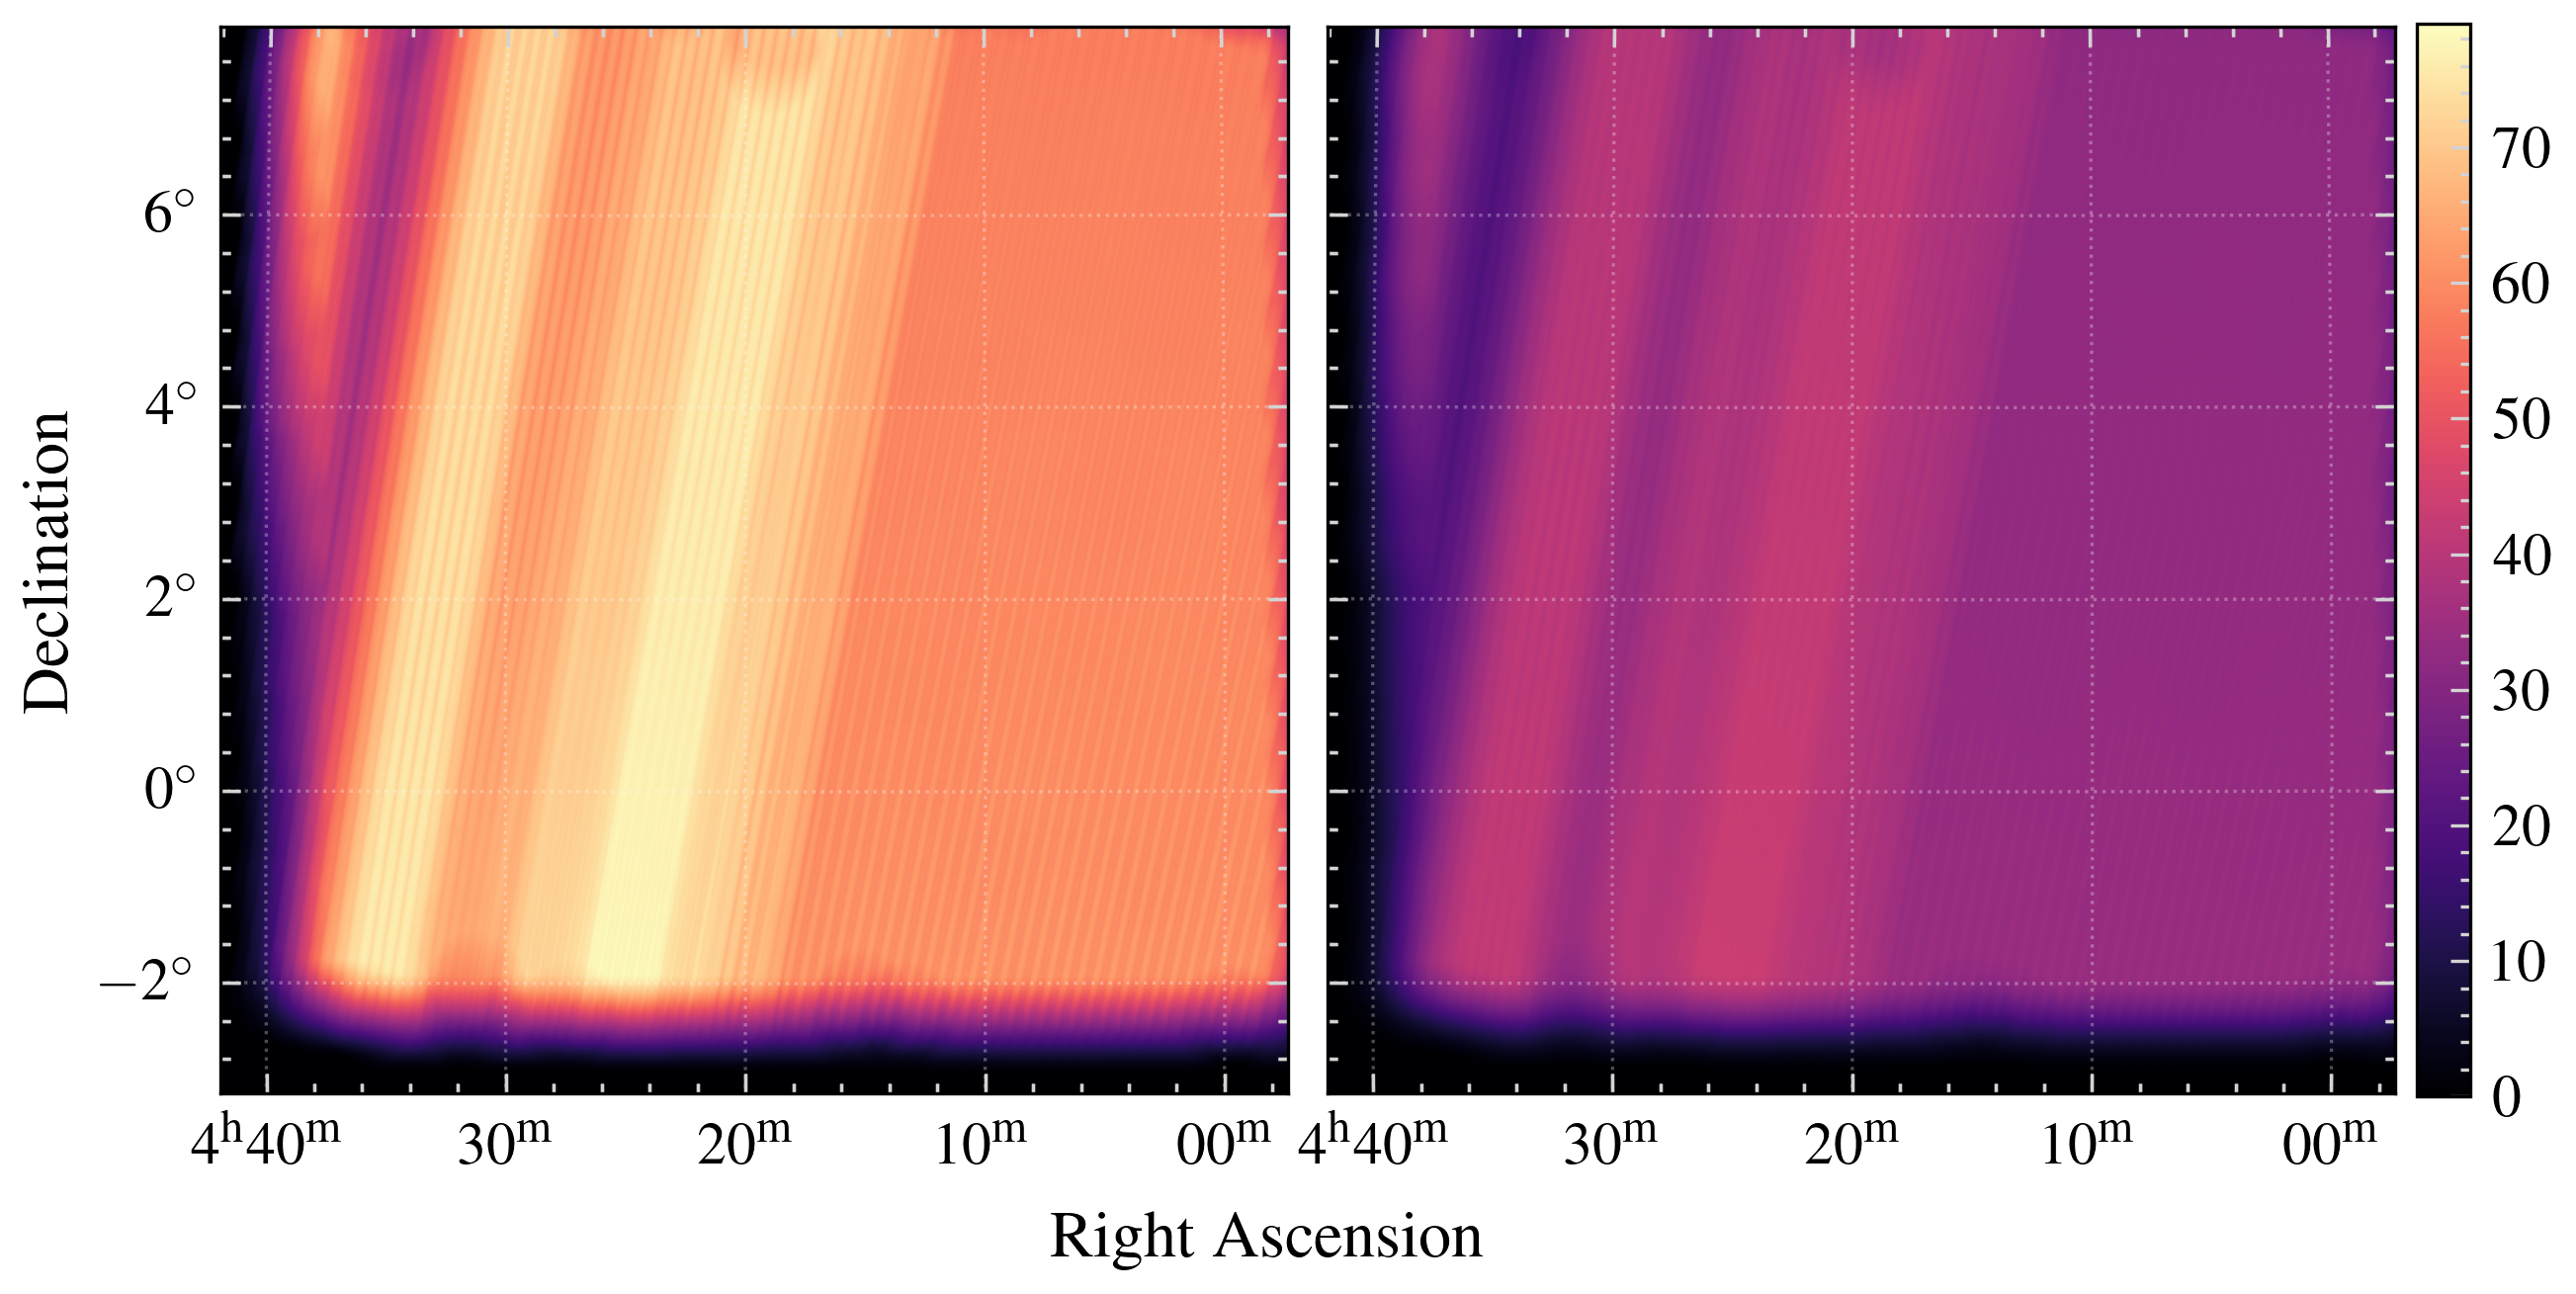
\includegraphics[width=\textwidth]{appendix_a/exposure_map_TM9.png}
    \caption[Exposure maps for TM9.]{Soft-bad exposure map for TM9 created in Section \ref{sec:exposure_map}. \textit{Left:} flat exposure map. \textit{Right:} vignetted exposure map. The color bar units are seconds.}
    \label{fig:TM9}
\end{figure}
%
\begin{figure}[htbp]
    \centering
    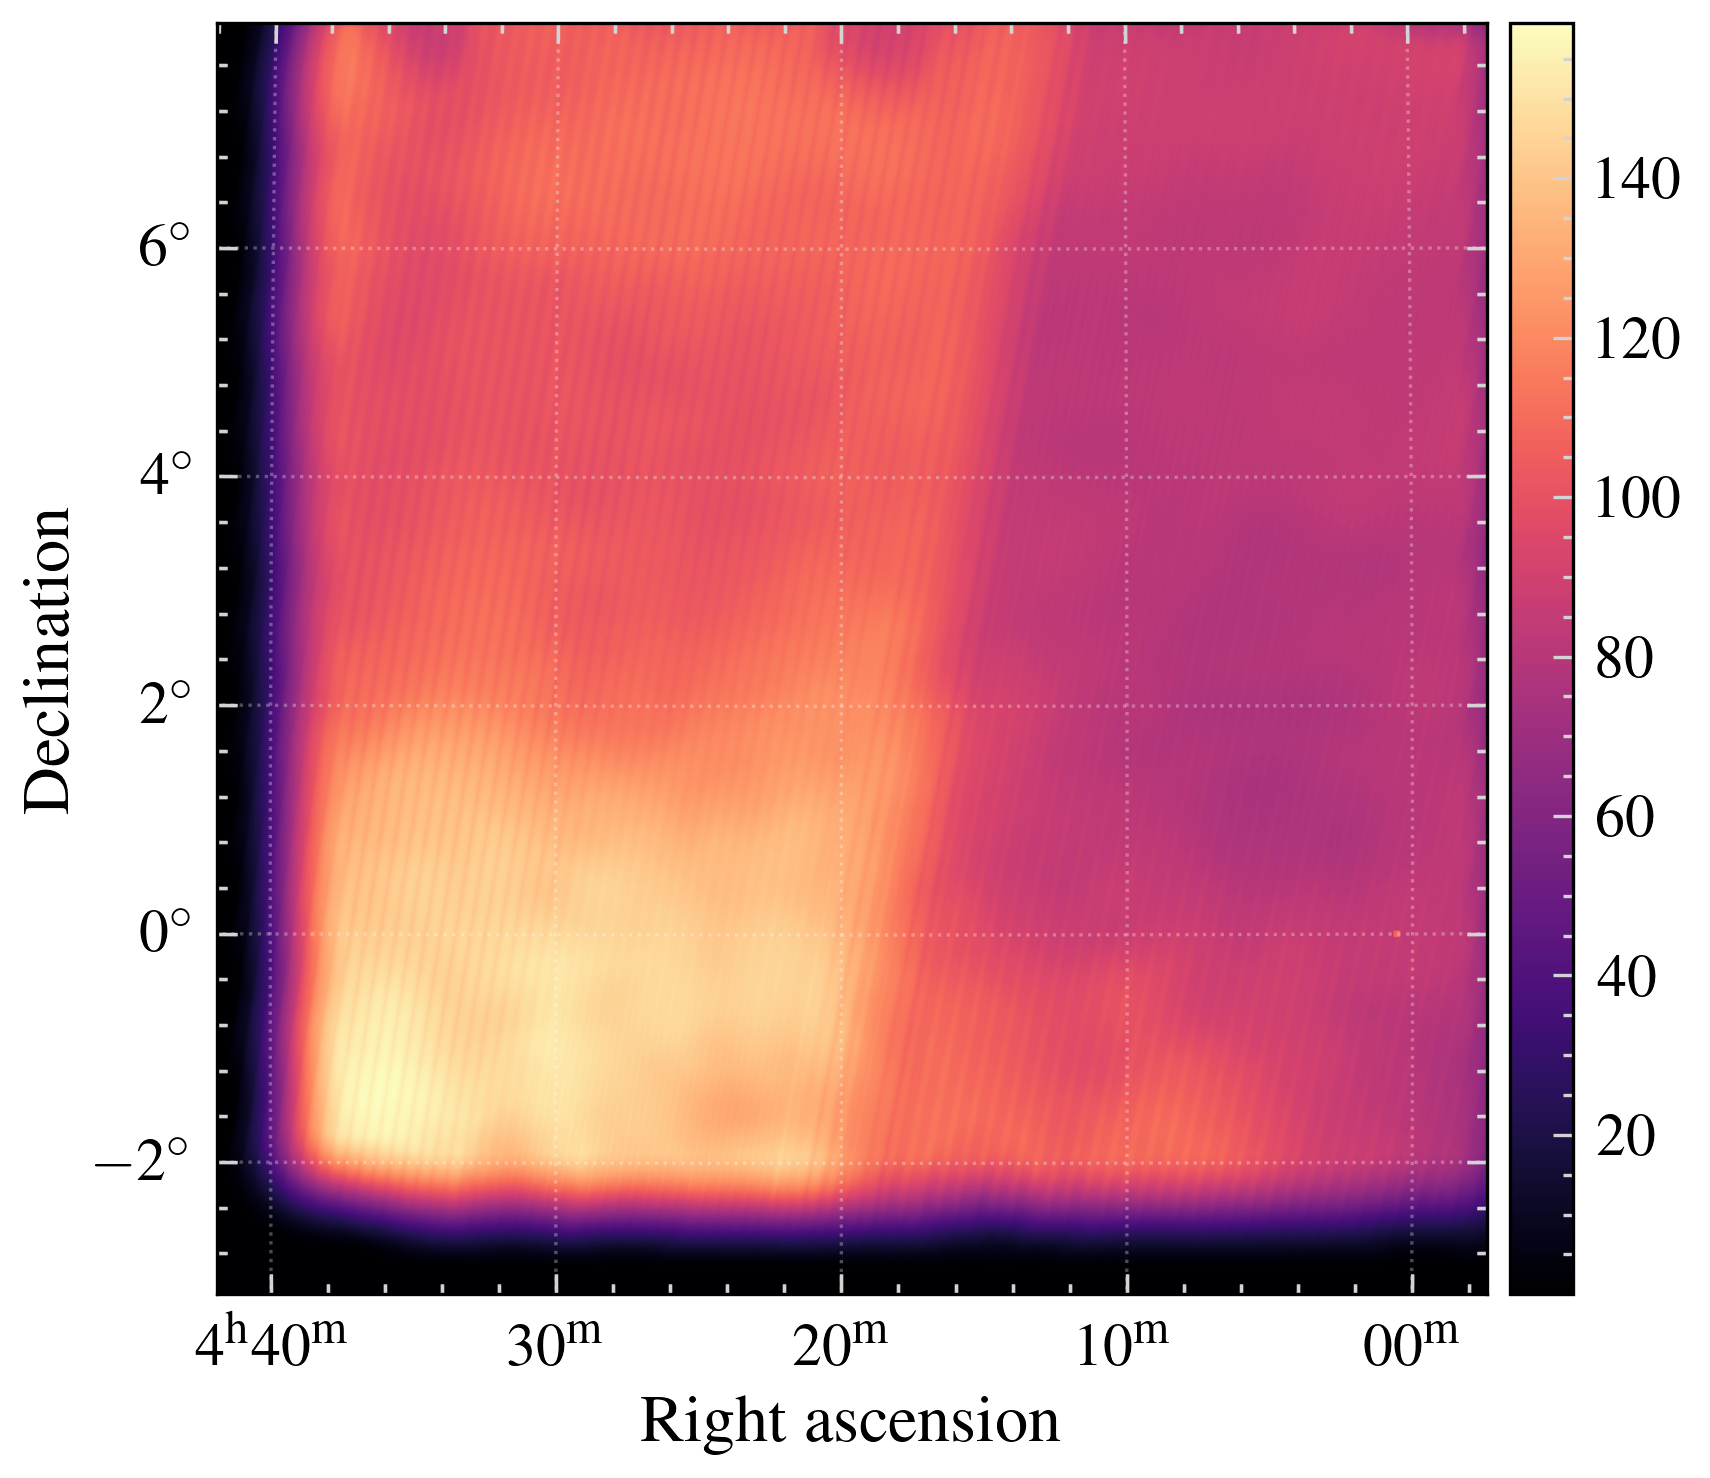
\includegraphics{appendix_a/exposure_map_TM0}
    \caption[Exposure maps for TM0.]{Fully corrected, soft-bad exposure map for TM0 obtained by the procedures outlined in Section \ref{sec:exposure}. \textit{Left:} flat exposure map. \textit{Right:} vignetted exposure map. The color bar units are seconds.}
    \label{fig:TM0}
\end{figure}
%
\clearpage
\section{PIB Map}\label{sec:appendix_a_pib_map}
\begin{figure}[htbp]
    \centering
    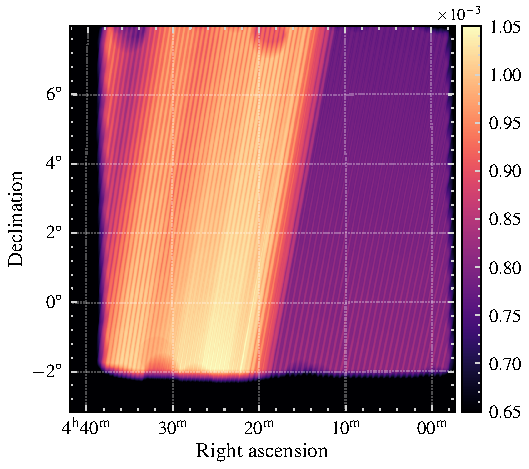
\includegraphics{data_reduction/PIB_MAP.pdf}
    \caption[PIB-map.]{PIB-map created by co-adding individual background maps for each telescope module (TM) as outlined in Section \ref{sec:pib_correction}.}
    \label{fig:pib_map}
\end{figure}
\begin{table}[htbp]
    \centering
    \begin{tabular}{ccc}
        \toprule
        TM & R & $H_\text{obs}$ \\ 
        \midrule
        1 & 1.30 & 9512 \\
        2 & 1.36 & 8362 \\
        3 & 1.35 & 9187 \\
        4 & 1.24 & 10177 \\
        5 & 0.85 & 10817 \\
        6 & 1.29 & 9144 \\
        7 & 0.82 & 10214 \\
        \bottomrule
    \end{tabular}
    \caption{Values of \(R\), and $H_\text{obs}$ utilized for the PIB-correction in Section \ref{sec:pib_correction}}
    \label{tab:values_of_R_and_H}
\end{table}
%
\clearpage
\section{Orion-Eridanus Superbubble}\label{sec:orion}
To better link the background gradient observed in the wavelet-filtered image (Figure \ref{fig:background_circles}) to the Orion-Eridanus superbubble, the ROSAT X-ray map of the Orion-Eridanus region presented by \citet{Krause_2014} and described in Section \ref{sec:background} was replaced by a cutout of the wavelet-filtered image at the position of NGC1550. For this, the orientation of the latter was changed to match the galactic coordinates present in the former. The result can be seen in Figure \ref{fig:superbubble_reprojected}. It is evident that the background gradient present in the eROSITA data lines up well with the gradient direction of the Orion-Eridanus superbubble.
\begin{figure}[htbp]
    \centering
    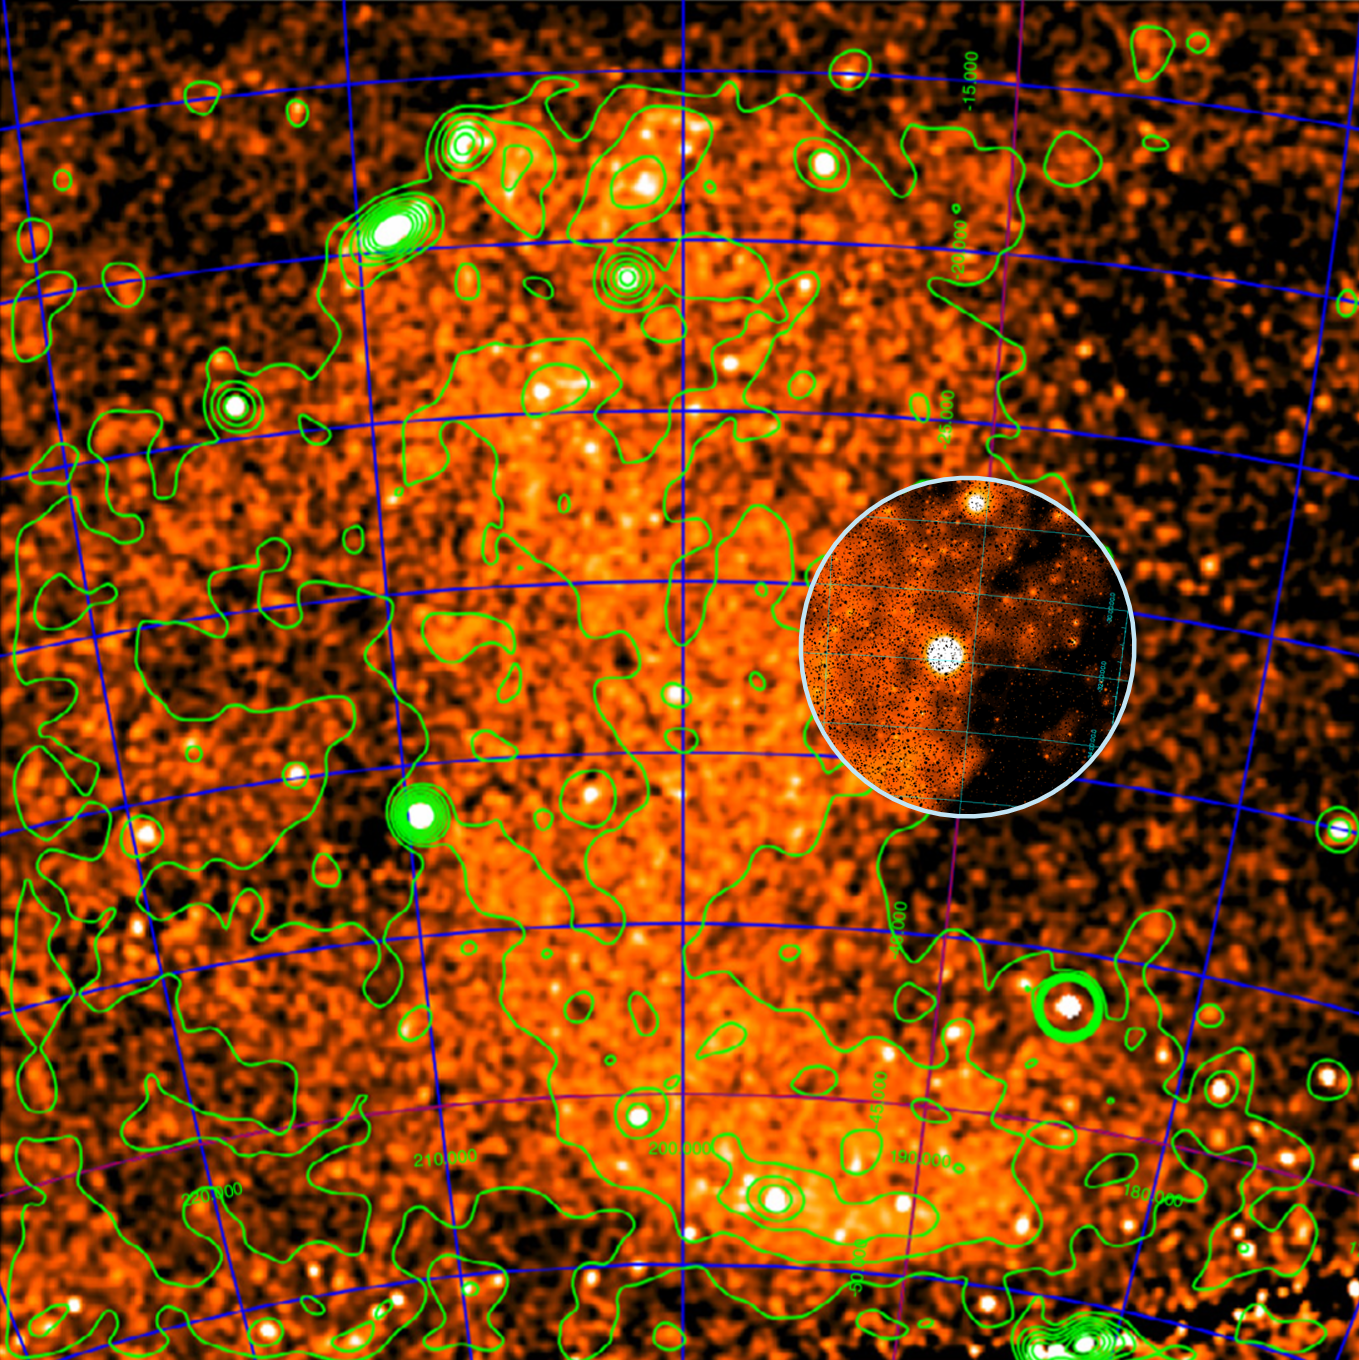
\includegraphics[height=0.66\textheight]{appendix_a/supper_bubble_reprojected.png}
    \caption[Reprojection of Wavelet-filtered image onto ROSAT X-ray map.]{Wavelet-filtered, soft-band image obtained in this thesis (white circle) cutout and reprojected onto the ROSAT X-ray map of the Orion-Eridanus superbubble taken from \citet{Krause_2014}. For visualization purposes, the color schemes were matched.}
    \label{fig:superbubble_reprojected}
\end{figure}